% ==========================================================
% 第13章 複素幾何と代数幾何
% ==========================================================
\chapter{複素幾何と代数幾何}
\label{ch:ch13}

\begin{chapterlead}
これまでの章では，代数多様体を多項式の零点集合として，すなわち「代数的」に扱ってきた．
基礎体が $\C$ のとき，代数多様体は同時に複素数の位相をもつ空間であり，局所的には正則関数で記述される
「複素多様体」（特異点があれば「複素解析的空間」）でもある．
本章ではこの二つの見方---代数的な見方と解析的な見方---を橋渡しする．
まず複素多様体と正則関数・正則写像の基礎を整理し，複素解析的空間を導入した後，
Chow の定理と GAGA の原理という「射影的な世界では代数と解析が一致する」という深い事実を紹介する．
最後に Riemann 面（1次元複素多様体）を詳しく調べ，2次元共形場理論と弦理論の世界面の幾何へとつなげる．
Kähler 幾何・Chern 類・標準束（canonical bundle）は第15章で，モジュライ空間は第16章で詳しく扱うので，
本章ではそれらには導入的に触れるにとどめる．
\end{chapterlead}

% ----------------------------------------------------------
\section{複素多様体の基礎}
% ----------------------------------------------------------

\subsection{複素座標}

$\C^n$ の点を $z=(z^1,\dots,z^n)$ と書き，各成分を実部・虚部に分けて
\begin{equation}
  z^j = x^j + i y^j,\qquad \bar z^{\bar j} = x^j - i y^j \qquad (j=1,\dots,n)
\end{equation}
とおく．これにより $\C^n\cong\R^{2n}$ と同一視される．
添字 $\bar j$ は「反正則な方向」であることを示すための記号であり，値としては $j$ と同じ範囲を動く．

微分作用素を
\begin{equation}
  \frac{\partial}{\partial z^j} = \frac12\left(\frac{\partial}{\partial x^j} - i\frac{\partial}{\partial y^j}\right),\qquad
  \frac{\partial}{\partial \bar z^{\bar j}} = \frac12\left(\frac{\partial}{\partial x^j} + i\frac{\partial}{\partial y^j}\right)
  \label{eq:ch13-wirtinger}
\end{equation}
と定める（Wirtinger 微分）．これらは
\begin{equation}
  \frac{\partial z^k}{\partial z^j}=\delta^k_j,\quad
  \frac{\partial \bar z^{\bar k}}{\partial z^j}=0,\quad
  \frac{\partial z^k}{\partial \bar z^{\bar j}}=0,\quad
  \frac{\partial \bar z^{\bar k}}{\partial \bar z^{\bar j}}=\delta^{k}_{j}
\end{equation}
をみたすように作られている．すなわち $z$ と $\bar z$ を「独立な変数」とみなして偏微分する形式的規則が正当化される．
1形式も $dz^j=dx^j+i\,dy^j$，$d\bar z^{\bar j}=dx^j-i\,dy^j$ とおけば，滑らかな関数 $f$ の外微分は
\begin{equation}
  df = \partial f + \bar\partial f,\qquad
  \partial f = \sum_j \frac{\partial f}{\partial z^j}dz^j,\quad
  \bar\partial f = \sum_j \frac{\partial f}{\partial \bar z^{\bar j}}d\bar z^{\bar j}
\end{equation}
と分解される．この $\partial,\bar\partial$ の分解が，以後の複素幾何のすべての出発点である．

\begin{myex}{1変数の場合}{ch13-wirtinger-ex}
$f(z)=z^2\bar z = |z|^2 z$ とすると $\partial f/\partial z = 2z\bar z$，$\partial f/\partial\bar z = z^2$．
後者が $0$ でないので，$f$ は正則でない（次節）．一方 $f(z)=e^{z}$ なら $\partial f/\partial\bar z=0$ である．
また $\Delta = \partial_x^2+\partial_y^2 = 4\,\partial_z\partial_{\bar z}$ が成り立つ．
\end{myex}

\subsection{複素ベクトル空間}

実ベクトル空間 $V$ 上の\textbf{複素構造}とは，線形写像 $J:V\to V$ で $J^2=-1$ をみたすものをいう．
$J$ を「$i$ 倍」と解釈すれば $V$ は複素ベクトル空間になり，$\dim_\R V = 2\dim_\C V$ である．
逆に複素ベクトル空間は，$i$ 倍写像を $J$ として実ベクトル空間と複素構造の組とみなせる．

$\R^{2n}=\C^n$ では，$J$ は
\begin{equation}
  J\frac{\partial}{\partial x^j}=\frac{\partial}{\partial y^j},\qquad J\frac{\partial}{\partial y^j}=-\frac{\partial}{\partial x^j}
\end{equation}
で与えられる．複素化 $V_\C=V\otimes_\R\C$ 上で $J$ は固有値 $\pm i$ をもち，
\begin{equation}
  V_\C = V^{1,0}\oplus V^{0,1},\qquad V^{1,0}=\{v: Jv = iv\},\quad V^{0,1}=\{v:Jv=-iv\}=\overline{V^{1,0}}
\end{equation}
と分解する．$\C^n$ では $V^{1,0}$ は $\partial/\partial z^j$ で，$V^{0,1}$ は $\partial/\partial\bar z^{\bar j}$ で張られる．
双対空間でも同様に $V_\C^*=(V^*)^{1,0}\oplus(V^*)^{0,1}$ となり，これから
$(p,q)$ 形式 $\bigwedge^{p,q}V^* = \bigwedge^p (V^*)^{1,0}\otimes\bigwedge^q (V^*)^{0,1}$ が定義される．
$(p,q)$ 形式は局所的に $dz^{i_1}\wedge\cdots\wedge dz^{i_p}\wedge d\bar z^{\bar j_1}\wedge\cdots\wedge d\bar z^{\bar j_q}$ の線形結合である．

\begin{note}
線形写像 $A:\C^n\to\C^m$ が $\C$-線形であることは，実線形写像として $AJ = JA$ をみたすことと同値である．
$\GL(n,\C)$ は $\GL(2n,\R)$ のうち $J$ と可換なもの全体であり，$\det_\R A = |\det_\C A|^2>0$．
特に複素線形同型は向きを保つ．これが「複素多様体は自然に向き付けられる」ことの理由である．
\end{note}

\subsection{複素多様体の定義}

\begin{mydef}{複素多様体}{ch13-cplx-mfd}
Hausdorff かつ第二可算な位相空間 $X$ が \textbf{$n$ 次元複素多様体}であるとは，
開被覆 $\{U_\alpha\}$ と同相写像 $\varphi_\alpha:U_\alpha\to\varphi_\alpha(U_\alpha)\subset\C^n$（開集合への）が与えられ，
$U_\alpha\cap U_\beta\neq\emptyset$ のとき座標変換
\begin{equation}
  \varphi_\beta\circ\varphi_\alpha^{-1}:\varphi_\alpha(U_\alpha\cap U_\beta)\to\varphi_\beta(U_\alpha\cap U_\beta)
\end{equation}
がすべて\textbf{正則}（双正則）であることをいう．$\{(U_\alpha,\varphi_\alpha)\}$ を正則座標近傍系（正則アトラス）といい，
同値な（合併がまた正則アトラスになる）アトラスの類を\textbf{複素構造}という．
\end{mydef}

実多様体の定義との違いは「座標変換が $C^\infty$」が「座標変換が正則」に置き換わった点だけである．
しかし，正則性は $C^\infty$ 性よりはるかに強い条件（Cauchy--Riemann 方程式という偏微分方程式系）であり，
このために複素多様体は実多様体よりずっと「硬い」．たとえば次の節で見るように，コンパクト複素多様体上の
正則関数は定数しかない．また，同じ実多様体の上に互いに同型でない複素構造が連続的に無数に存在しうる
（トーラスの例，第16章のモジュライ）．

$n$ 次元複素多様体は $2n$ 次元の向き付けられた実多様体であり，各点の接空間 $T_pX$ には
座標によらない複素構造 $J_p$ が定まる（座標変換の Jacobi 行列が $\C$-線形であるため）．
この $J$ を\textbf{概複素構造}という．逆に $J^2=-1$ をみたす $J$ がいつ複素構造から来るかは
Newlander--Nirenberg の定理（積分可能性条件 $N_J=0$）が答えるが，本ノートでは扱わない．

\subsection{複素多様体の局所座標}

正則座標 $(z^1,\dots,z^n)$ と別の正則座標 $(w^1,\dots,w^n)$ が重なる領域では $w=w(z)$ は正則であるから
\begin{equation}
  dw^i = \frac{\partial w^i}{\partial z^j}dz^j,\qquad d\bar w^{\bar i} = \overline{\frac{\partial w^i}{\partial z^j}}\,d\bar z^{\bar j}
\end{equation}
となり，$dz$ と $d\bar z$ は混ざらない（以後，上下に同じ添字が現れたら和をとる）．
したがって $(p,q)$ 形式の概念は座標によらず定義され，
\begin{equation}
  \Omega^k(X)\otimes\C = \bigoplus_{p+q=k}\Omega^{p,q}(X)
\end{equation}
という分解が大域的に意味をもつ．外微分も $d=\partial+\bar\partial$，$\partial:\Omega^{p,q}\to\Omega^{p+1,q}$，
$\bar\partial:\Omega^{p,q}\to\Omega^{p,q+1}$ と分解し，$d^2=0$ から
\begin{equation}
  \partial^2=0,\qquad \bar\partial^2 = 0,\qquad \partial\bar\partial+\bar\partial\partial=0
\end{equation}
が従う．$\bar\partial^2=0$ から Dolbeault コホモロジー $H^{p,q}_{\bar\partial}(X)=\Ker\bar\partial/\Img\bar\partial$ が定義されるが，
その詳細とHodge理論は第15章に譲る．

正則な座標変換の Jacobi 行列 $(\partial w^i/\partial z^j)$ に対し，実 Jacobi 行列式は
$|\det(\partial w/\partial z)|^2>0$ であるから，すべての座標変換が向きを保つ．
\begin{note}
$(n,0)$ 形式 $dz^1\wedge\cdots\wedge dz^n$ は座標変換で $\det(\partial z/\partial w)$ 倍される．この変換則をもつ
直線束が標準束 $K_X$ であり，Calabi--Yau 条件 $K_X\cong\OO_X$ の舞台となる（第15章）．
\end{note}

\subsection{複素多様体の例}

\begin{myex}{$\C^n$ とその開集合}{ch13-cn}
$\C^n$ 自身，およびその開集合は，恒等写像1枚の座標で複素多様体である．
\end{myex}

\begin{myex}{複素射影空間 $\PP^n$}{ch13-cpn}
$\PP^n=\C\PP^n = (\C^{n+1}\setminus\{0\})/\C^*$ を同次座標 $[Z_0:\cdots:Z_n]$ で表す．
$U_\alpha=\{Z_\alpha\neq0\}$ 上の座標を $z_{(\alpha)}^{k}=Z_k/Z_\alpha$（$k\neq\alpha$）とすると，
$U_\alpha\cap U_\beta$ での座標変換は
\begin{equation}
  z_{(\beta)}^k = \frac{Z_k}{Z_\beta} = \frac{z^k_{(\alpha)}}{z^\beta_{(\alpha)}}\qquad(z^\alpha_{(\alpha)}:=1)
\end{equation}
であり，$z^\beta_{(\alpha)}\neq0$ の領域で正則である．よって $\PP^n$ は $n$ 次元のコンパクト複素多様体である
（コンパクト性は $S^{2n+1}\subset\C^{n+1}\setminus\{0\}$ からの全射連続写像の像であることから）．
$n=1$ の場合 $\PP^1$ は座標 $z$ と $w=1/z$ の2枚で覆われる Riemann 球面 $S^2$ である．
\end{myex}

\begin{myex}{複素トーラス}{ch13-torus}
$\Lambda\subset\C^n$ を，$\R$ 上一次独立な $2n$ 個のベクトルで生成される格子とする．
$\Lambda$ は平行移動で $\C^n$ に自由かつ真性不連続に作用し，商 $T=\C^n/\Lambda$ は位相的には $(S^1)^{2n}$ である．
平行移動 $z\mapsto z+\lambda$ は正則なので，$\C^n$ の座標が局所座標を与え，$T$ はコンパクト複素多様体になる．
$n=1$，$\Lambda=\Z\omega_1+\Z\omega_2$（$\Img(\omega_2/\omega_1)>0$）のとき，基本領域は図\ref{fig:ch13-torus}の平行四辺形であり，
向かい合う辺を貼り合わせるとドーナツ型の曲面が得られる．
\end{myex}

\begin{figure}[ht]
\centering
\begin{tikzpicture}[scale=1.1]
  \draw[->,gray] (-0.5,0)--(3.6,0) node[right]{$\Re z$};
  \draw[->,gray] (0,-0.5)--(0,2.3) node[above]{$\Img z$};
  \fill[blue!8] (0,0)--(2,0)--(2.8,1.6)--(0.8,1.6)--cycle;
  \draw[thick,blue!70!black,-{Stealth}] (0,0)--(2,0) node[midway,below]{$\omega_1$};
  \draw[thick,blue!70!black,-{Stealth}] (0,0)--(0.8,1.6) node[midway,left]{$\omega_2$};
  \draw[thick,blue!70!black,dashed] (2,0)--(2.8,1.6);
  \draw[thick,blue!70!black,dashed] (0.8,1.6)--(2.8,1.6);
  \foreach \i in {0,1} \foreach \j in {-1,0,1} {
    \fill ({2*\i+0.8*\j},{1.6*\j}) circle (1pt);}
  \node at (1.4,0.8) {$F$};
  % torus
  \begin{scope}[xshift=6cm,yshift=0.8cm]
    \draw[thick] (0,0) ellipse (1.6 and 0.8);
    \draw[thick] (-0.7,0.05) .. controls (-0.3,-0.25) and (0.3,-0.25) .. (0.7,0.05);
    \draw[thick] (-0.55,-0.05) .. controls (-0.2,0.15) and (0.2,0.15) .. (0.55,-0.05);
    \draw[red!70!black,thick] (0,-0.2) arc[start angle=90,end angle=270,x radius=0.12,y radius=0.3];
    \draw[red!70!black,thick,dashed] (0,-0.8) arc[start angle=-90,end angle=90,x radius=0.12,y radius=0.3];
    \node[red!70!black] at (0.35,-0.55) {$a$};
    \draw[green!50!black,thick] (0,0) ellipse (1.15 and 0.52);
    \node[green!50!black] at (1.25,0.45) {$b$};
  \end{scope}
  \draw[->,thick] (3.4,0.8)--(4.2,0.8) node[midway,above]{\small 貼り合わせ};
\end{tikzpicture}
\caption{格子 $\Lambda=\Z\omega_1+\Z\omega_2$ と基本領域 $F$．$F$ の対辺を同一視して得られるトーラス $\C/\Lambda$．$a,b$ は1次ホモロジーの生成元．}
\label{fig:ch13-torus}
\end{figure}

$\C/\Lambda$ は実多様体としてはどれも $S^1\times S^1$ だが，複素多様体としては格子の「形」に依存する．
$\Lambda$ を $\omega_1^{-1}$ 倍しても（正則な線形変換なので）同型は変わらないので，$\Lambda=\Z+\Z\tau$，
$\tau=\omega_2/\omega_1\in\mathbb{H}=\{\Img\tau>0\}$ と正規化できる．さらに基底の取り替え
\begin{equation}
  \tau\mapsto \frac{a\tau+b}{c\tau+d},\qquad \begin{pmatrix}a&b\\c&d\end{pmatrix}\in\SL(2,\Z)
  \label{eq:ch13-modular}
\end{equation}
は同じ格子を与えるので，複素トーラスの同型類は $\mathbb{H}/\SL(2,\Z)$ の点と一対一に対応する．
$\tau$ を\textbf{モジュラーパラメータ}と呼ぶ．これは第16章で扱う「モジュライ空間」の最も基本的な例であり，
13.6節で弦理論のトーラス振幅に再登場する．

\begin{myex}{射影超曲面}{ch13-hypersurface}
$F(Z_0,\dots,Z_{n+1})$ を次数 $d$ の同次多項式とし，$X=\{F=0\}\subset\PP^{n+1}$ が非特異（$\partial F/\partial Z_k$ が
$X$ 上で同時には消えない）とする．正則版の陰関数定理により，各点の近傍で $n$ 個の正則座標がとれ，$X$ は $n$ 次元
コンパクト複素多様体になる．たとえば $d=3$ の平面曲線（楕円曲線），$\PP^4$ 内の 5 次超曲面（quintic Calabi--Yau，第15章）がある．
\end{myex}

\begin{physbox}[複素座標と場の理論]
2次元 Euclid 場の理論では世界面座標 $(\sigma^1,\sigma^2)$ を $z=\sigma^1+i\sigma^2$ にまとめるのが標準的である．
$\partial_z,\partial_{\bar z}$ は光錐座標 $\partial_\pm$ の Euclid 版であり，Laplacian $4\partial\bar\partial$ が
左右に分解することが「左向き・右向きの運動」の分離（13.6節）を意味する．
\end{physbox}

\exprob{ch13-pr-p1}
$\PP^1$ の2つの座標近傍 $U_0=\{Z_0\neq0\}$，$U_1=\{Z_1\neq0\}$ で，座標 $z=Z_1/Z_0$，$w=Z_0/Z_1$ をとる．
1形式 $dz$ を $w$ で書き直し，$\PP^1$ 上に至るところ零でない正則1形式が存在しないことを示せ．

\exprob{ch13-pr-gl}
$A\in M_n(\C)$ を $\R^{2n}$ 上の実線形写像とみたときの行列式が $|\det A|^2$ であることを示せ．
（ヒント：$A$ を上三角化せよ．）

% ----------------------------------------------------------
\section{正則関数と正則写像}
% ----------------------------------------------------------

\subsection{正則関数}

\begin{mydef}{正則関数}{ch13-holfn}
開集合 $U\subset\C^n$ 上の $C^1$ 級関数 $f:U\to\C$ が\textbf{正則}であるとは，
\begin{equation}
  \frac{\partial f}{\partial \bar z^{\bar j}} = 0\qquad (j=1,\dots,n),\quad\text{すなわち}\quad \bar\partial f=0
  \label{eq:ch13-cr}
\end{equation}
が成り立つことをいう．複素多様体 $X$ 上の関数は，各正則座標で表したとき正則であるとき正則という．
$X$ の開集合 $U$ 上の正則関数全体を $\OO_X(U)$ と書き，これにより $X$ 上の\textbf{正則関数の層} $\OO_X$ が定まる．
\end{mydef}

$f=u+iv$ と書くと，\eqref{eq:ch13-cr} は各変数について
\begin{equation}
  \frac{\partial u}{\partial x^j}=\frac{\partial v}{\partial y^j},\qquad
  \frac{\partial u}{\partial y^j}=-\frac{\partial v}{\partial x^j}
\end{equation}
という \textbf{Cauchy--Riemann 方程式}と同値である．すなわち $f$ の実 Jacobi 行列が $J$ と可換（$\C$-線形）であることを意味する．

1変数の場合に知られている基本性質は次のとおりである：
(i) 正則関数は Cauchy の積分公式
\begin{equation}
  f(z) = \frac{1}{2\pi i}\oint_{|\zeta-a|=r}\frac{f(\zeta)}{\zeta - z}\,d\zeta\qquad(|z-a|<r)
\end{equation}
をみたし，特に収束冪級数に展開される（解析的）．
(ii) \textbf{一致の定理}：連結領域上の正則関数が空でない開集合上で $0$ なら恒等的に $0$．
(iii) \textbf{最大値原理}：連結領域上で $|f|$ が内点で最大値をとれば $f$ は定数．
(iv) \textbf{Liouville の定理}：$\C$ 全体で有界な正則関数は定数．

\begin{myex}{正則と非正則}{ch13-holex}
多項式 $p(z)$，$e^z$，$\sin z$ は $\C$ 上正則．$1/z$ は $\C\setminus\{0\}$ 上正則．
$\bar z$，$|z|^2$，$\Re z$ は正則でない．実数値の正則関数は（連結領域上で）定数である（Cauchy--Riemann から $du=0$）．
\end{myex}

\subsection{多変数複素解析の基礎}

多変数の正則関数も，多重円板 $\Delta(a;r)=\{|z^j-a^j|<r_j\}$ 上で反復 Cauchy 積分公式
\begin{equation}
  f(z) = \frac{1}{(2\pi i)^n}\oint_{|\zeta^1-a^1|=r_1}\!\!\cdots\oint_{|\zeta^n-a^n|=r_n}
  \frac{f(\zeta)\,d\zeta^1\cdots d\zeta^n}{(\zeta^1-z^1)\cdots(\zeta^n-z^n)}
\end{equation}
をみたし，冪級数に展開される．したがって一致の定理・最大値原理・Liouville の定理は多変数でも成り立つ．
（実は各変数ごとに正則でありさえすれば，連続性を仮定せずとも多変数正則になる：Hartogs の定理．）

しかし多変数では1変数にない全く新しい現象が起こる．その代表が次である．

\begin{mythm}{Hartogs の拡張定理}{ch13-hartogs}
$n\geq2$ とし，$U\subset\C^n$ を開集合，$K\subset U$ をコンパクト集合で $U\setminus K$ が連結とする．
このとき $U\setminus K$ 上の任意の正則関数は $U$ 上の正則関数に一意的に拡張される．
特に $\C^n\setminus\{0\}$（$n\geq 2$）上の正則関数は $\C^n$ 全体に拡張される．
\end{mythm}

\begin{proof}[証明の概略（原点を除いた多重円板の場合）]
$n=2$，$f$ が $\Delta\setminus\{0\}$（$\Delta=\{|z^1|<1,|z^2|<1\}$）で正則とする．$0<r<1$ を固定し
\begin{equation}
  F(z^1,z^2) = \frac{1}{2\pi i}\oint_{|\zeta|=r}\frac{f(z^1,\zeta)}{\zeta - z^2}\,d\zeta \qquad(|z^2|<r)
\end{equation}
とおく．積分路上 $(z^1,\zeta)\neq0$ なので被積分関数は $z^1$ について正則で，$F$ は $\{|z^1|<1,|z^2|<r\}$ 全体で正則である．
一方 $z^1\neq0$ を固定すると $\zeta\mapsto f(z^1,\zeta)$ は円板 $|\zeta|<1$ 全体で正則なので，1変数の Cauchy 公式より $F(z^1,z^2)=f(z^1,z^2)$．
一致の定理により $F$ は $f$ の拡張を与える．
\end{proof}

1変数では $1/z$ のように孤立特異点をもつ正則関数が存在するのに対し，2変数以上では
「点（さらには余次元2以上の集合）だけを除いた所で正則な関数」は自動的にそこまで延びてしまう．
この結果，\textbf{多変数正則関数の零点集合や極集合は孤立点にならず，必ず余次元1}（超曲面）である．
実際 $f$ が孤立零点 $p$ をもてば $1/f$ が $p$ を除いて正則となり，Hartogs により $p$ まで延びて矛盾する．
これは代数幾何で「因子は余次元1」であることや，Krull の主イデアル定理の解析版にあたる．

\begin{note}
Hartogs 現象は $\C^n$ の開集合の中に「正則関数で区別できない」形のものがあることを意味し，
正則関数の自然な定義域（正則領域・Stein 多様体）の理論へつながる．アフィン代数多様体の解析化は Stein 多様体の典型例である．
\end{note}

\subsection{正則写像}

\begin{mydef}{正則写像}{ch13-holmap}
複素多様体の間の連続写像 $f:X\to Y$ が\textbf{正則写像}であるとは，局所座標で表したとき各成分が正則関数であることをいう．
同値な言い方として，任意の開集合 $V\subset Y$ と $g\in\OO_Y(V)$ に対し $g\circ f\in\OO_X(f^{-1}V)$ となること（引き戻し $f^*:\OO_Y\to f_*\OO_X$）．
正則な逆写像をもつ正則全単射を\textbf{双正則写像}という．
\end{mydef}

正則写像 $f$ の微分 $df_p:T_pX\to T_{f(p)}Y$ は $J$ と可換であり，複素 Jacobi 行列 $(\partial f^i/\partial z^j)$ で表される．
逆関数定理・陰関数定理の正則版が成り立つ：$\det(\partial f^i/\partial z^j)(p)\neq0$ なら $f$ は $p$ の近傍で双正則．
また1変数では正則な全単射は自動的に双正則であり，多変数でも同じことが成り立つ（Osgood の定理）．

\begin{myex}{正則写像の例}{ch13-holmap-ex}
(1) $\C^{n+1}\setminus\{0\}\to\PP^n$，$Z\mapsto[Z]$ は正則．
(2) Veronese 写像 $\PP^1\to\PP^2$，$[s:t]\mapsto[s^2:st:t^2]$ は正則で，像は円錐曲線 $Z_0Z_2=Z_1^2$．
(3) 射影 $\C\to\C/\Lambda$ は正則な被覆写像．
(4) $\PP^1$ の自己双正則写像は1次分数変換 $z\mapsto (az+b)/(cz+d)$ であり，$\Aut(\PP^1)=\PGL(2,\C)$．
\end{myex}

\subsection{正則写像の局所性}

正則関数・正則写像はその\textbf{局所的な振る舞いが大域的な振る舞いを決めてしまう}．
これが複素幾何を代数幾何に近づける最大の要因である．

\begin{myprop}{コンパクト複素多様体上の正則関数}{ch13-cpt-const}
$X$ を連結なコンパクト複素多様体とする．このとき $X$ 上の正則関数は定数に限る：$\OO_X(X)=\C$．
\end{myprop}

\begin{proof}
$f\in\OO_X(X)$ とする．$|f|$ は連続でありコンパクト集合上で最大値をある点 $p$ でとる．
$p$ の座標近傍で最大値原理を用いると $f$ は $p$ の近傍で定数 $c=f(p)$ である．
$\{x\in X: f\equiv c \text{ が } x \text{ の近傍で成り立つ}\}$ は空でない開集合であり，
一致の定理（座標近傍ごとに適用）により閉集合でもある．$X$ は連結なのでこれは $X$ 全体である．
\end{proof}

この命題は，代数幾何における「射影多様体上の大域正則関数は定数」に対応する（第10章参照）．
コンパクト複素多様体上では「関数」が少なすぎるので，代わりに\textbf{有理型関数}や
\textbf{直線束の正則切断}（第14章）を考えることになる．たとえば $\PP^n$ 上の大域正則関数は定数だが，
次数 $d$ の同次多項式は直線束 $\OO(d)$ の正則切断として豊富に存在する．

\begin{mycor}{}{ch13-cpt-map}
連結コンパクト複素多様体 $X$ から $\C^m$ への正則写像は定数写像である．
特に $\dim X\geq1$ のコンパクト複素多様体は $\C^m$ の閉複素部分多様体にはならない．
\end{mycor}

この系は，コンパクトな対象を扱うには $\C^m$ ではなく $\PP^m$ のような「コンパクトな周囲空間」が必要であることを示している．
これが射影幾何が複素幾何において中心的である理由である．

\subsection{正則関数と代数的構造}

$\PP^n$ 上では正則関数は定数だけだったが，\textbf{有理型関数}（局所的に正則関数の商 $g/h$ で $h\not\equiv0$）は豊富にある．
たとえば同じ次数の同次多項式の商 $P(Z)/Q(Z)$ は $\PP^n$ 上の有理型関数を与える．
実は逆も成り立つ：

\begin{mythm}{}{ch13-mero-pn}
$\PP^n$ 上の有理型関数はすべて，同じ次数の同次多項式の商 $P/Q$ で表される．
すなわち，$\PP^n$ の有理型関数体は有理関数体 $\C(z^1,\dots,z^n)$ と一致する．
\end{mythm}

この定理は「解析的な対象（有理型関数）が実は代数的である」という主張の最初の例である．
1変数の場合を確かめよう．$f$ を $\PP^1$ 上の有理型関数とする．極はコンパクト性から有限個 $a_1,\dots,a_k$（$\infty$ を含むかもしれない）．
各有限の極 $a_j$ での主要部 $\sum_{m=1}^{N_j}c_{j,m}(z-a_j)^{-m}$ を差し引き，$\infty$ での主要部（$z$ の多項式）も差し引くと，
$\PP^1$ 全体で正則な関数が残り，命題\ref{prop:ch13-cpt-const}により定数である．よって $f$ は有理関数である．

一般に，$n$ 次元コンパクト連結複素多様体 $X$ の有理型関数体 $\mathcal{M}(X)$ の超越次数は $n$ 以下であり
（Siegel の定理），等号が成り立つものを Moishezon 多様体と呼ぶ．射影代数多様体ではつねに等号が成り立ち，
$\mathcal{M}(X)$ は代数多様体としての有理関数体 $\C(X)$ と一致する．
一方，一般の複素トーラス $\C^n/\Lambda$（$n\geq2$）では有理型関数が定数しかないこともあり，
このようなトーラスは射影代数多様体にならない．\textbf{すべての複素多様体が代数的なわけではない}ことに注意しよう．

\exprob{ch13-pr-zero}
$n\geq2$ とする．$\C^n$ 上の正則関数 $f$ の零点集合が孤立点 $p$ を含まないことを，Hartogs の定理を用いて示せ．

\exprob{ch13-pr-aut}
$\C/\Lambda$ から $\PP^1$ への正則写像で定数でないものが存在するなら，それは全射であることを示せ．
（ヒント：正則写像の像の開性と，コンパクト性．）

% ----------------------------------------------------------
\section{複素解析的空間}
% ----------------------------------------------------------

\subsection{複素解析的集合}

\begin{mydef}{複素解析的集合}{ch13-analytic-set}
複素多様体 $X$ の部分集合 $A$ が\textbf{（複素）解析的集合}であるとは，$A$ が閉集合であり，
各点 $p\in X$ に近傍 $U$ と有限個の正則関数 $f_1,\dots,f_k\in\OO_X(U)$ が存在して
\begin{equation}
  A\cap U = \{x\in U : f_1(x)=\cdots=f_k(x)=0\}
\end{equation}
と書けることをいう．
\end{mydef}

これは代数的集合（多項式の共通零点，第3章）の「局所版」であり，多項式の代わりに正則関数を，
大域的な方程式の代わりに局所的な方程式を許したものである．
代数的集合は解析的集合だが，逆は一般に成り立たない．

\begin{myex}{代数的でない解析的集合}{ch13-nonalg}
$\C^2$ 内の $A=\{(z,w): w = e^z\}$ は解析的集合（正則関数 $w-e^z$ の零点）であるが，代数的集合ではない．
実際，直線 $w=1$ との交わり $\{(2\pi i k,1):k\in\Z\}$ は無限個の点からなるが，代数曲線と直線の交わりは
（直線を含まない限り）有限個である．$\C^n$ のような非コンパクトな空間では「無限遠での振る舞い」が
代数性を壊すのである．
\end{myex}

解析的集合も既約成分への分解，次元，特異点集合といった代数的集合と同様の概念をもつ．
局所的には，$p\in A$ における正則関数の芽の環 $\OO_{X,p}$（収束冪級数環 $\C\{z^1,\dots,z^n\}$）は
Noether 局所環かつ一意分解整域であり（Weierstrass の準備定理から従う），
$A$ の芽の局所構造は $\OO_{X,p}$ のイデアル論で記述される．

\subsection{局所的な解析的構造}

局所的な解析を支える基本道具が次の定理である．

\begin{mythm}{Weierstrass の準備定理}{ch13-wpt}
$f\in\C\{z^1,\dots,z^{n-1},w\}$ が $f(0,w)=w^d\cdot(\text{単元})$ をみたすとする（$w$ 方向に位数 $d$）．
このとき原点の近くで一意的に
\begin{equation}
  f = u\cdot\left(w^d + a_1(z)w^{d-1}+\cdots+a_d(z)\right),\qquad u(0)\neq0,\ a_k(0)=0
\end{equation}
と分解される．括弧内を Weierstrass 多項式という．
\end{mythm}

すなわち，局所的には任意の正則関数の零点集合は「$z$ をパラメータとする $w$ の $d$ 次多項式の根」として記述できる．
これにより $f=0$ は $z$-空間上の $d$ 重分岐被覆となり，解析的集合の局所構造が代数的な多項式の議論に帰着する．
たとえば $f(z,w)=w^2-z^3$ は原点近傍で $z$ 平面上の2重分岐被覆 $w=\pm z^{3/2}$ であり，原点で分岐する（尖点）．

\begin{myex}{局所既約性}{ch13-node}
$A=\{w^2=z^2(z+1)\}\subset\C^2$ は代数的には既約（多項式 $w^2-z^3-z^2$ は既約）である．
しかし原点の近くでは $\sqrt{z+1}$ が正則関数として定まるので
\begin{equation}
  w^2 - z^2(z+1) = \bigl(w - z\sqrt{1+z}\bigr)\bigl(w+z\sqrt{1+z}\bigr)
\end{equation}
と分解し，原点の芽としては2つの成分（2本の滑らかな枝）をもつ．
すなわち\textbf{代数的に既約でも解析的に局所可約}になりうる．これが「結節点（node）」の局所像である．
\end{myex}

\subsection{複素解析的空間}

複素多様体は局所的に $\C^n$ の開集合をモデルとした．特異点を許すには，局所モデルを解析的集合に取り替えればよい．
ただしスキーム（第12章）と同様に，点集合だけでなく「関数の層」を込めて考えるのが正しい．

\begin{mydef}{複素解析的空間}{ch13-analytic-space}
\textbf{局所モデル}とは，開集合 $U\subset\C^n$，連接なイデアル層 $\sheaf{I}=(f_1,\dots,f_k)\subset\OO_U$ に対し，
$A=\{f_1=\cdots=f_k=0\}$ と環の層 $\OO_A = (\OO_U/\sheaf{I})|_A$ の組 $(A,\OO_A)$ をいう．
\textbf{複素解析的空間}とは，$\C$-代数の局所環つき空間 $(X,\OO_X)$ であって，各点が局所モデルと同型な近傍をもつものをいう．
\end{mydef}

これは「アフィンスキームを貼り合わせたものがスキーム」という定義（第12章）と全く平行である：
\begin{center}
\begin{tabular}{c|c}
代数幾何 & 複素解析幾何 \\ \hline
多項式環 $\C[z^1,\dots,z^n]$ & 収束冪級数環 $\C\{z^1,\dots,z^n\}$ / 正則関数の層 \\
アフィンスキーム $\Spec A$ & 局所モデル $(A,\OO_U/\sheaf{I})$ \\
スキーム & 複素解析的空間 \\
連接層 & 連接解析的層
\end{tabular}
\end{center}
層を込めるので，$\{z^2=0\}$ のような「非被約」な構造（点としては $\{z=0\}$ だが関数として $z\neq0$, $z^2=0$）も扱える．
連接性については Oka の連接定理（$\OO_{\C^n}$ が連接層であること）が基礎となる．

\subsection{特異複素解析的空間}

解析的空間 $X$ の点 $p$ が\textbf{非特異（正則点）}であるとは，$p$ の近傍が複素多様体（局所モデルとして $\OO_U$ そのもの）
と同型であることをいい，そうでない点を\textbf{特異点}という．局所モデル $\{f_1=\cdots=f_k=0\}$ では，
Jacobi 行列 $(\partial f_i/\partial z^j)$ の階数が $n-\dim_pX$ に一致する点が非特異点である（被約な場合）．
これは代数的集合の非特異性の Jacobi 判定法（第7章）と同じ形である．

\begin{myex}{代表的な特異点}{ch13-sing}
(1) 尖点 $\{w^2=z^3\}\subset\C^2$：原点で特異．正規化 $t\mapsto (t^2,t^3)$ は全単射だが双正則ではない．
(2) 結節点 $\{zw=0\}$：2本の直線の交わり．
(3) $A_1$ 特異点（円錐） $\{x^2+y^2+z^2=0\}\subset\C^3$，あるいは同値な商 $\C^2/\{\pm1\}$．
Calabi--Yau の特異点・解消の局所モデルとして第15章・第17章（conifold）で重要になる．
\end{myex}

特異点の集合 $\Sing X$ は $X$ の解析的部分集合であり，$X$ の中で「薄い」（至るところ稠密でない）．
広中の特異点解消定理により，任意の（被約な）複素解析的空間は，特異点の上でのみ変更を加える
固有写像 $\tilde X\to X$（特異点の外では双正則）によって非特異化できる．

\exprob{ch13-pr-cusp}
尖点 $C=\{w^2=z^3\}\subset\C^2$ について，写像 $\nu:\C\to C$，$t\mapsto(t^2,t^3)$ が同相写像であるが，
逆写像が正則でないことを示せ．また $\nu^*:\OO_{C,0}\to\OO_{\C,0}$ の像が $\C\{t^2,t^3\}$ であることを確かめよ．

% ----------------------------------------------------------
\section{複素多様体と代数多様体}
% ----------------------------------------------------------

\subsection{代数多様体から複素多様体へ}

$\C$ 上の代数多様体 $X$（たとえば $\C^n$ や $\PP^n$ の中の代数的集合）には，Zariski 位相とは別に，
$\C^n$ の通常の位相から誘導される\textbf{古典位相}（Euclid 位相）が入る．
さらに，正則関数の層を（多項式を正則関数とみて）入れることで，複素解析的空間 $X^{\rm an}$ が得られる．
これを $X$ の\textbf{解析化}という．

\begin{myprop}{解析化}{ch13-analytification}
$\C$ 上の代数多様体（より一般に有限型スキーム）$X$ に対し，複素解析的空間 $X^{\rm an}$ が自然に定まり，次をみたす．
(1) $X^{\rm an}$ の点集合は $X$ の閉点（$\C$-値点）の集合である．
(2) $X$ が非特異なら $X^{\rm an}$ は $\dim_\C X$ 次元の複素多様体である．
(3) 射 $f:X\to Y$ は正則写像 $f^{\rm an}:X^{\rm an}\to Y^{\rm an}$ を誘導する（関手性）．
(4) $X$ が完備（たとえば射影的）なら $X^{\rm an}$ はコンパクトである．
\end{myprop}

(2) は代数的な Jacobi 判定法と正則版陰関数定理による．Zariski 位相は古典位相よりずっと粗い
（Zariski 開集合は古典位相で開かつ稠密）ことに注意しよう．たとえば $\A^1$ の Zariski 開集合は有限集合の補集合のみであり，
円板のような「小さい」近傍は存在しない．解析化することで初めて，$\C$ の局所的な解析（冪級数展開，積分，ホモトピー）が使えるようになる．

\begin{figure}[ht]
\centering
\begin{tikzcd}[column sep=large, row sep=large]
  \text{代数多様体 } X \arrow[r, "(\cdot)^{\rm an}"] \arrow[d, "f"'] & \text{複素解析的空間 } X^{\rm an} \arrow[d, "f^{\rm an}"] \\
  \text{代数多様体 } Y \arrow[r, "(\cdot)^{\rm an}"'] & \text{複素解析的空間 } Y^{\rm an}
\end{tikzcd}
\caption{解析化の関手性}
\end{figure}

\subsection{代数的構造と解析的構造}

解析化によって代数多様体は複素解析的空間に移されるが，その逆を問うことができる：
\begin{itemize}
  \item 複素解析的空間（あるいはその部分集合）はいつ代数的か？
  \item 解析化の際に「情報が増える」ことはあるか？ たとえば解析的には同型だが代数的には同型でない2つの多様体はあるか？
  \item 正則写像・正則関数・正則ベクトル束はいつ代数的なものから来るか？
\end{itemize}
非コンパクトな場合はこれらの答えは否定的である．$e^z$ は $\A^1$ 上の正則関数だが多項式ではなく，
例\ref{ex:ch13-nonalg} の $\{w=e^z\}$ は代数的でない．さらに，$\C^*$ と $\C$ 上の「穴あき円板」の比較や，
代数的には異なるが解析的に同型なアフィン曲面の例も知られている．
非コンパクトな解析的世界は，代数的世界よりもはるかに広い．

これに対し，\textbf{射影的（コンパクト）}な場合には驚くべきことに答えが肯定的になる．
大雑把に言えば，コンパクト性が「無限遠での振る舞い」を制限し，冪級数が多項式で打ち切られることを強制するのである
（$\PP^1$ 上の有理型関数が有理関数になる議論，定理\ref{thm:ch13-mero-pn} を思い出そう）．

\subsection{射影代数多様体と複素多様体}

\begin{mythm}{Chow の定理}{ch13-chow}
$\PP^n$ の任意の閉複素解析的部分集合は代数的集合である．すなわち，有限個の同次多項式の共通零点として表される．
\end{mythm}

\begin{proof}[証明のアイデア（超曲面の場合）]
$A\subset\PP^n$ が余次元1の解析的集合とし，錐 $\hat A=\pi^{-1}(A)\cup\{0\}\subset\C^{n+1}$ を考える．
$\hat A$ はスカラー倍で不変な解析的集合である．原点の近傍で $\hat A$ を定義する正則関数 $f$ を冪級数展開
$f=\sum_d f_d$（$f_d$ は $d$ 次同次多項式）すると，$\hat A$ のスカラー倍不変性から各 $f_d$ が $\hat A$ 上で消えることが
示され，$\hat A$（したがって $A$）は同次多項式の零点で定まる．一般の場合は射影と次元に関する帰納法を用いる．
（スカラー倍で原点の近傍が全体に広がるという点で，コンパクト性＝錐構造が本質的に効いている．）
\end{proof}

Chow の定理の系として，次が得られる：
\begin{itemize}
  \item $\PP^n$ に正則に埋め込まれたコンパクト複素多様体は射影代数多様体である．
  \item 射影代数多様体の間の正則写像は代数的な射である（グラフが $\PP^n\times\PP^m$ の解析的部分集合で，Segre 埋め込みにより Chow の定理が適用できる）．
  \item 射影代数多様体の間で，解析的同型と代数的同型は一致する．
\end{itemize}

Chow の定理を大きく一般化したのが Serre の GAGA（Géométrie Algébrique et Géométrie Analytique, 1956）である．

\begin{mythm}{GAGA}{ch13-gaga}
$X$ を $\C$ 上の射影代数多様体（射影スキーム）とする．このとき
\begin{enumerate}
  \item 解析化 $\sheaf{F}\mapsto\sheaf{F}^{\rm an}$ は，$X$ 上の連接代数的層の圏から $X^{\rm an}$ 上の連接解析的層の圏への\textbf{圏同値}を与える．
  \item 任意の連接層 $\sheaf{F}$ と $q\geq0$ に対し，コホモロジーの自然な写像
  \begin{equation}
    H^q(X,\sheaf{F})\xrightarrow{\ \sim\ } H^q(X^{\rm an},\sheaf{F}^{\rm an})
  \end{equation}
  は同型である．
\end{enumerate}
\end{mythm}

この定理の意味を噛み砕くと次のようになる．
\begin{itemize}
  \item （1）の「本質的全射性」：射影多様体上の任意の正則ベクトル束（第14章）は代数的ベクトル束から来る．たとえば $\PP^n$ 上の正則直線束は $\OO(d)$ に限られ，$\Pic(\PP^n)\cong\Z$ は解析的にも正しい．
  \item （1）の「充満忠実性」：代数的な束の間の正則な準同型は自動的に代数的である．
  \item （2）：大域正則切断 $H^0$ の次元や，Riemann--Roch 定理に現れる $H^1$ などのコホモロジーは，代数的に計算しても解析的に計算しても同じである．
\end{itemize}
したがって，物理で現れる「正則な対象（正則切断，ゼロモード，正則ベクトル束）」が射影多様体上のものである限り，
それらは完全に代数的に（多項式とイデアルで）扱える．逆に，代数的な対象について解析的な道具（調和形式，曲率積分，
指数定理）を用いて結論を得ることも正当化される．

\subsection{解析的な方法と代数的な方法}

GAGA の恩恵により，射影多様体については二つの方法を自由に行き来できる．それぞれの長所を比較しておこう．

\textbf{解析的な方法}：
\begin{itemize}
  \item 計量（Hermitian 計量，Kähler 計量）を入れて微分幾何の道具が使える．調和形式による Hodge 分解（第15章）．
  \item 曲率の積分として位相不変量（Chern 類）を表せる．Gauss--Bonnet，指数定理．
  \item 位相（基本群，ホモロジー，周期積分）を直接扱える．周期 $\oint_\gamma\Omega$ による複素構造の記述．
  \item ゲージ理論の偏微分方程式（Hermitian--Yang--Mills 方程式，第14章）を解くことができる．
\end{itemize}

\textbf{代数的な方法}：
\begin{itemize}
  \item 多項式の方程式として具体的に書け，計算機で扱える（Gröbner 基底など）．
  \item 任意の体（有限体，$p$ 進体）上で意味をもち，数論と結びつく．
  \item 特異点や非被約構造，族（モジュライ）の扱いがスキーム論で統一的にできる．
  \item 安定性・GIT 商のような「代数的」な条件でモジュライを構成できる（第14章の小林--Hitchin 対応は，これを解析的条件と結びつける）．
\end{itemize}

\begin{myex}{楕円曲線の二つの顔}{ch13-two-faces}
楕円曲線は，代数的には $\PP^2$ 内の非特異3次曲線 $y^2=4x^3-g_2x-g_3$ であり，解析的には複素トーラス $\C/\Lambda$ である．
両者を結ぶのが Weierstrass の $\wp$ 関数である（13.5.4節）．代数的な顔からは群法則の多項式公式や $j$ 不変量が，
解析的な顔からは周期 $\omega_1,\omega_2$，モジュラーパラメータ $\tau$ と $\SL(2,\Z)$ 作用が見える．
\end{myex}

\subsection{代数幾何と複素幾何の相互関係}

ここまでの関係を図式にまとめる．
\begin{center}
\begin{tikzpicture}[every node/.style={draw,rounded corners,align=center,font=\small,inner sep=4pt}]
  \node (proj) at (0,0) {射影代数多様体};
  \node (kahler) at (5,0) {コンパクト Kähler 多様体};
  \node (cpt) at (10,0) {コンパクト複素多様体};
  \node (alg) at (0,-2) {代数多様体（一般）};
  \node (an) at (10,-2) {複素解析的空間};
  \draw[-{Stealth}] (proj)--(kahler) node[midway,above,draw=none]{\scriptsize Fubini--Study 計量};
  \draw[-{Stealth}] (kahler)--(cpt);
  \draw[-{Stealth}] (alg)--(an) node[midway,above,draw=none]{\scriptsize 解析化 $X\mapsto X^{\rm an}$};
  \draw[-{Stealth}] (proj)--(alg);
  \draw[-{Stealth}] (cpt)--(an);
\end{tikzpicture}
\end{center}
包含関係はすべて真である：
\begin{itemize}
  \item 射影代数多様体は $\PP^n$ の Fubini--Study 計量を制限することで Kähler 多様体になる（第15章）．
  \item 一般の複素トーラス $\C^2/\Lambda$ は Kähler（平坦計量）だが射影的でない．射影的になる条件は Riemann の双線形関係（偏極の存在）で与えられる．
  \item Hopf 曲面 $(\C^2\setminus\{0\})/\langle z\mapsto 2z\rangle\cong S^1\times S^3$ はコンパクト複素多様体だが，$b_1=1$ が奇数なので Kähler でない．
\end{itemize}
Kähler 多様体が射影的になるための判定条件として，小平の埋め込み定理がある：
コンパクト Kähler 多様体 $X$ が射影的であるための必要十分条件は，正の直線束（曲率が正）をもつこと，
すなわち Kähler 類を整数係数のコホモロジー類に選べることである（Hodge 多様体）．これは第15章の Chern 類の言葉で述べられる．

物理的には，Calabi--Yau 多様体は一般にはKähler 多様体として定義されるが，興味のある多くの例（quintic など）は
射影的であり，GAGA によって代数的手法（多項式の変形 = 複素構造の変形，第16章）が適用できる．

\begin{physbox}[代数と解析の往来]
弦理論のコンパクト化で現れる無質量粒子の数は，内部空間上のコホモロジー $H^q(X,\sheaf{F})$ の次元で数えられる．
物理的には「調和形式（Laplacian のゼロモード）」として解析的に定義されるが，Hodge 理論と GAGA によって
これは代数的な層コホモロジーと一致し，多項式の計算で求められる．たとえば quintic の複素構造変形の数 $101$ は，
5次多項式の係数の数から $\GL(5,\C)$ の次元を引いた $126-25=101$ として代数的に数えられる（第15章・第16章）．
\end{physbox}

\exprob{ch13-pr-chow}
$\C^2$ の解析的集合 $\{w=e^z\}$ は代数的でない（例\ref{ex:ch13-nonalg}）．これは Chow の定理と矛盾しないことを，
$\PP^2$ における閉包を考えることで説明せよ．

\exprob{ch13-pr-hopf}
Hopf 曲面 $X=(\C^2\setminus\{0\})/\langle z\mapsto 2z\rangle$ が $S^1\times S^3$ と微分同相であることを示せ．

% ----------------------------------------------------------
\section{Riemann面}
% ----------------------------------------------------------

\subsection{Riemann面の定義}

\begin{mydef}{Riemann 面}{ch13-riemann-surface}
連結な1次元複素多様体を \textbf{Riemann 面}という．
\end{mydef}

Riemann 面は実2次元の向き付けられた曲面である．コンパクトな向き付け可能曲面は位相的に
\textbf{種数（genus）} $g$（「穴の数」，ハンドルの数）で完全に分類され，Euler 標数は
\begin{equation}
  \chi = 2-2g
\end{equation}
である．1次ホモロジーは $H_1(\Sigma_g,\Z)\cong\Z^{2g}$ で，標準的な生成元 $a_1,\dots,a_g,b_1,\dots,b_g$
（交点数 $a_i\cdot b_j=\delta_{ij}$）をとることができる．

\begin{figure}[ht]
\centering
\begin{tikzpicture}[scale=0.8]
  % genus 0
  \draw[thick] (0,0) circle (1);
  \draw[dashed] (-1,0) arc[start angle=180,end angle=0,x radius=1,y radius=0.3];
  \draw (-1,0) arc[start angle=180,end angle=360,x radius=1,y radius=0.3];
  \node at (0,-1.6) {$g=0$（$\PP^1$）};
  % genus 1
  \begin{scope}[xshift=4cm]
    \draw[thick] (0,0) ellipse (1.6 and 1);
    \draw[thick] (-0.6,0.05) .. controls (-0.25,-0.25) and (0.25,-0.25) .. (0.6,0.05);
    \draw[thick] (-0.45,-0.05) .. controls (-0.15,0.15) and (0.15,0.15) .. (0.45,-0.05);
    \node at (0,-1.6) {$g=1$（楕円曲線）};
  \end{scope}
  % genus 2
  \begin{scope}[xshift=9.5cm]
    \draw[thick] (0,0) ellipse (2.3 and 1);
    \foreach \c in {-1,1} {
      \draw[thick] (\c-0.5,0.05) .. controls (\c-0.2,-0.25) and (\c+0.2,-0.25) .. (\c+0.5,0.05);
      \draw[thick] (\c-0.38,-0.04) .. controls (\c-0.12,0.13) and (\c+0.12,0.13) .. (\c+0.38,-0.04);
    }
    \draw[red!70!black,thick] (-1,0.0) ellipse (0.8 and 0.4);
    \node[red!70!black] at (-1,0.6) {\scriptsize $b_1$};
    \draw[green!50!black,thick] (-1,-0.2) arc[start angle=90,end angle=270,x radius=0.1,y radius=0.36];
    \node[green!50!black] at (-0.7,-0.65) {\scriptsize $a_1$};
    \node at (0,-1.6) {$g=2$};
  \end{scope}
\end{tikzpicture}
\caption{コンパクト Riemann 面の位相型（種数 $g=0,1,2$ の模式図）}
\label{fig:ch13-genus}
\end{figure}

\begin{myex}{Riemann 面の例}{ch13-rs-ex}
(1) $\C$，単位円板 $\mathbb{D}$，上半平面 $\mathbb{H}$（$\mathbb{D}\cong\mathbb{H}$）．
(2) Riemann 球面 $\PP^1$（$g=0$）．
(3) 複素トーラス $\C/\Lambda$（$g=1$）．
(4) 非特異平面代数曲線 $\{F=0\}\subset\PP^2$（13.5.3節）．
(5) 多価関数 $w=\sqrt{(z-e_1)(z-e_2)\cdots(z-e_{2g+2})}$ を1価にする Riemann 面（超楕円曲線，種数 $g$）．
\end{myex}

\subsection{複素構造}

同じ位相曲面上に，互いに双正則でない複素構造が多数ありうる．これを扱うのが\textbf{一意化定理}である．

\begin{mythm}{一意化定理}{ch13-uniformization}
単連結な Riemann 面は $\PP^1$，$\C$，$\mathbb{H}$ のいずれかに双正則である．
したがって任意の Riemann 面 $\Sigma$ は，その普遍被覆 $\tilde\Sigma\in\{\PP^1,\C,\mathbb{H}\}$ の
自己同型群の離散部分群 $\Gamma$（自由に作用）による商 $\tilde\Sigma/\Gamma$ として表される．
\end{mythm}

コンパクトな場合には次のように種数で振り分けられる：
\begin{center}
\begin{tabular}{c|c|c|c}
種数 & 普遍被覆 & 定曲率計量 & 例 \\ \hline
$g=0$ & $\PP^1$ & 正曲率（球面） & $\PP^1$ のみ \\
$g=1$ & $\C$ & 平坦 & $\C/\Lambda$ \\
$g\geq2$ & $\mathbb{H}$ & 負曲率（双曲） & $\mathbb{H}/\Gamma$，$\Gamma\subset\mathrm{PSL}(2,\R)$
\end{tabular}
\end{center}
（ここで $\mathrm{PSL}(2,\R)=\SL(2,\R)/\{\pm1\}$．）
特に種数0のコンパクト Riemann 面は $\PP^1$ ただ一つであり，種数1のものは $\C/\Lambda$ で尽くされる．

\textbf{複素構造と共形構造}：向き付けられた曲面上では，複素構造を与えることと共形構造（計量の局所的な
スケール倍 $g\sim e^{2\sigma}g$ の同値類）を与えることは同値である．実際，計量は局所的に等温座標で
$ds^2 = e^{2\sigma}(dx^2+dy^2)=e^{2\sigma}|dz|^2$ と書け，等温座標どうしの向きを保つ座標変換は共形写像＝正則写像である．
この事実が，2次元共形場理論と Riemann 面の幾何を直結させる（13.6節）．

種数 $g$ の複素構造の同値類全体（モジュライ空間 $\mathcal{M}_g$）の次元は
\begin{equation}
  \dim_\C \mathcal{M}_g = \begin{cases} 0 & g=0\\ 1 & g=1\\ 3g-3 & g\geq2\end{cases}
\end{equation}
である．$g=1$ の場合は $\tau\in\mathbb{H}/\SL(2,\Z)$ であった．モジュライ空間の構成と変形理論は第16章で扱う．

\subsection{射影曲線}

非特異な射影代数曲線は Riemann 面であり，逆に（Riemann の存在定理により）任意のコンパクト Riemann 面は
射影曲線として $\PP^N$ に埋め込める．GAGA と合わせて，
\begin{center}
\textbf{コンパクト Riemann 面} $=$ \textbf{非特異射影代数曲線}
\end{center}
という同一視が成り立つ．代数曲線論と Riemann 面論は同じものの二つの顔である．

平面曲線の種数は次数だけで決まる．

\begin{mythm}{種数公式}{ch13-genus-formula}
$C\subset\PP^2$ を次数 $d$ の非特異平面曲線とすると，その種数は
\begin{equation}
  g = \frac{(d-1)(d-2)}{2}.
\end{equation}
\end{mythm}

\begin{proof}[証明（Riemann--Hurwitz による）]
適当に座標をとり，点 $[0:1:0]\notin C$ とし，そこからの射影 $\pi:C\to\PP^1$，$[X:Y:Z]\mapsto[X:Z]$ を考える．
一般の $[X:Z]$ 上で $F(X,Y,Z)=0$ は $Y$ についての $d$ 次方程式なので，$\pi$ は $d$ 重被覆である．
分岐点は $F=\partial F/\partial Y=0$ をみたす点であり，Bézout の定理（第9章）により一般的な座標で $d(d-1)$ 個，
各々の分岐指数は $2$（単純分岐）である．Riemann--Hurwitz の公式
\begin{equation}
  \chi(C) = d\cdot\chi(\PP^1) - \sum_{p}(e_p-1)
\end{equation}
より $2-2g = 2d - d(d-1)$，すなわち $g=(d^2-3d+2)/2=(d-1)(d-2)/2$．
\end{proof}

\begin{center}
\begin{tabular}{c|cccccc}
$d$ & 1 & 2 & 3 & 4 & 5 & 6\\ \hline
$g$ & 0 & 0 & 1 & 3 & 6 & 10
\end{tabular}
\end{center}
直線と円錐曲線は $\PP^1$，3次曲線は楕円曲線，4次曲線は種数3である．
種数2の曲線は平面曲線としては非特異に実現できず（$g=2$ は $(d-1)(d-2)/2$ の値にならない），
超楕円曲線 $w^2=\prod_{k=1}^6(z-e_k)$ として実現される．
なお特異点をもつ平面曲線では，結節点・尖点1個ごとに種数（正規化の種数）が1ずつ減る．

\begin{note}
Riemann--Hurwitz 公式は，$\pi:C\to\PP^1$ に適合する $\PP^1$ の三角形分割を $C$ に引き戻すと，
分岐点以外では各セルが $d$ 枚に増えることから従う．分岐点 $p$ では $d$ 枚のうち $e_p$ 枚が1点に潰れるため，
頂点の数が $e_p-1$ だけ減る．
\end{note}

\subsection{楕円曲線}

種数1のコンパクト Riemann 面 $E=\C/\Lambda$，$\Lambda=\Z\omega_1+\Z\omega_2$ を考える．
$E$ 上の有理型関数は，$\C$ 上の二重周期的有理型関数（楕円関数）
$f(z+\omega_1)=f(z+\omega_2)=f(z)$ にほかならない．命題\ref{prop:ch13-cpt-const}により，正則な楕円関数は定数である．
また基本領域の境界に沿った積分で，楕円関数の留数の和は $0$ であることがわかるので，
基本領域にただ1つの1位の極をもつ楕円関数は存在しない．最も簡単な非自明な楕円関数は2位の極をもつ．

\begin{mydef}{Weierstrass の $\wp$ 関数}{ch13-wp}
\begin{equation}
  \wp(z) = \frac{1}{z^2} + \sum_{\lambda\in\Lambda\setminus\{0\}}\left(\frac{1}{(z-\lambda)^2}-\frac{1}{\lambda^2}\right).
\end{equation}
\end{mydef}

この級数は $\Lambda$ 上で広義一様に絶対収束し（$\sum_{\lambda\neq0}|\lambda|^{-3}<\infty$ による），
$\wp$ は偶関数で，各格子点に2位の極をもつ楕円関数である．
（周期性は $\wp'(z)=-2\sum_\lambda(z-\lambda)^{-3}$ が明らかに周期的であることと，偶関数性から従う．）
原点のまわりで Laurent 展開すると，
\begin{equation}
  \wp(z) = \frac{1}{z^2} + \frac{g_2}{20}z^2 + \frac{g_3}{28}z^4 + O(z^6),\qquad
  g_2 = 60\sum_{\lambda\neq0}\frac{1}{\lambda^4},\quad g_3 = 140\sum_{\lambda\neq0}\frac{1}{\lambda^6}.
\end{equation}

\begin{mythm}{$\wp$ の微分方程式と3次曲線への埋め込み}{ch13-wp-cubic}
$\wp$ は
\begin{equation}
  (\wp')^2 = 4\wp^3 - g_2\wp - g_3
  \label{eq:ch13-wp-ode}
\end{equation}
をみたす．さらに写像
\begin{equation}
  \Phi: \C/\Lambda\to\PP^2,\qquad z\mapsto [\wp(z):\wp'(z):1]\ (z\notin\Lambda),\quad 0\mapsto[0:1:0]
\end{equation}
は，$E=\C/\Lambda$ から非特異3次曲線 $Y^2Z = 4X^3 - g_2XZ^2 - g_3Z^3$ への双正則写像である．
\end{mythm}

\begin{proof}[証明の概略]
Laurent 展開から $(\wp')^2 = 4z^{-6} - \tfrac{2g_2}{5}z^{-2}-\tfrac{4g_3}{7}+O(z^2)$，
$4\wp^3 = 4z^{-6}+\tfrac{3g_2}{5}z^{-2}+\tfrac{3g_3}{7}+O(z^2)$ であるから，
$(\wp')^2-4\wp^3+g_2\wp+g_3$ は原点で正則かつ $0$ になる楕円関数である．よって定数 $0$．

$\Phi$ が well-defined かつ正則であること：$z\to0$ では同次座標に $z^3$ を掛けると $[z^3\wp:z^3\wp^{\prime}:z^3]\to[0:-2:0]=[0:1:0]$ となり，$0$ の近傍でも正則に延びる．
単射性：$\wp$ は基本領域で2位の極を1つもつので，各値をちょうど2回（重複込み）とる．
$\wp$ は偶関数なので $\wp(z)=\wp(-z)$ であり，$\wp(z_1)=\wp(z_2)$ なら $z_2\equiv\pm z_1$．
このとき $\wp'$ は奇関数なので $\wp'(z_2)=\pm\wp'(z_1)$ となり，$(\wp,\wp')$ は $z$ を区別する
（$z\equiv-z$ となる半周期点では $\wp'=0$ となり矛盾は生じない）．
曲線の非特異性は，右辺 $4x^3-g_2x-g_3$ の3根 $e_k=\wp(\omega_k/2)$（$\omega_3=\omega_1+\omega_2$）が相異なることから従う．
$\Phi$ はコンパクト Riemann 面の間の単射正則写像なので全射でもあり，双正則である．
\end{proof}

判別式 $\Delta = g_2^3-27g_3^2\neq0$ が非特異性の条件であり，$j$ 不変量
\begin{equation}
  j(\tau) = 1728\frac{g_2^3}{g_2^3-27g_3^2}
\end{equation}
は格子の $\C^*$ 倍で不変，かつ \eqref{eq:ch13-modular} の $\SL(2,\Z)$ 変換で不変であり，
$j:\mathbb{H}/\SL(2,\Z)\to\C$ は全単射を与える．すなわち \textbf{楕円曲線の同型類は $j$ 不変量で分類される}．
楕円曲線の群構造（3次曲線の弦-接線法と $\C/\Lambda$ の加法の一致），モジュライは第16章，F 理論への応用は第17章で扱う．

\begin{figure}[ht]
\centering
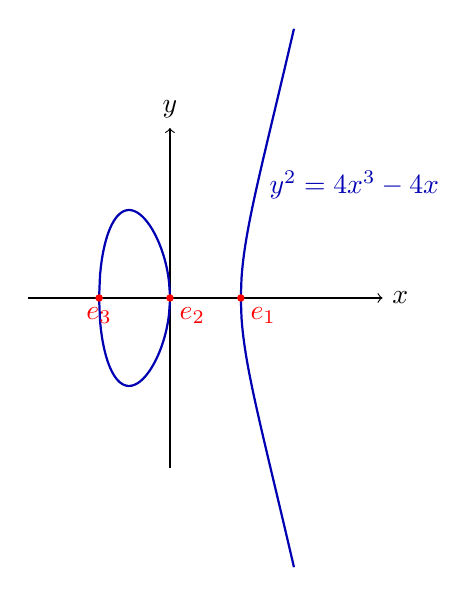
\begin{tikzpicture}[scale=0.9]
  \draw[->] (-2,0)--(3,0) node[right]{$x$};
  \draw[->] (0,-2.4)--(0,2.4) node[above]{$y$};
  \draw[thick,blue!70!black,domain=-1.0:-0.0,samples=80] plot ({\x},{sqrt(max(0,4*\x*\x*\x-4*\x))});
  \draw[thick,blue!70!black,domain=-1.0:-0.0,samples=80] plot ({\x},{-sqrt(max(0,4*\x*\x*\x-4*\x))});
  \draw[thick,blue!70!black,domain=1.0:1.75,samples=80] plot ({\x},{sqrt(4*\x*\x*\x-4*\x)});
  \draw[thick,blue!70!black,domain=1.0:1.75,samples=80] plot ({\x},{-sqrt(4*\x*\x*\x-4*\x)});
  \node[blue!70!black] at (2.6,1.6) {$y^2=4x^3-4x$};
  \foreach \e in {-1,0,1} \fill[red] (\e,0) circle (1.5pt);
  \node[below,red] at (-1,0) {$e_3$};
  \node[below right,red] at (0,0) {$e_2$};
  \node[below right,red] at (1,0) {$e_1$};
\end{tikzpicture}
\caption{実3次曲線 $y^2=4x^3-g_2x-g_3$（$g_2=4,g_3=0$）の実部分．半周期点 $\omega_k/2$ は $y=0$ の3点 $e_k$ に，原点 $0\in\C/\Lambda$ は無限遠点 $[0:1:0]$ に移る．}
\end{figure}

\subsection{Riemann面と物理}

Riemann 面上の正則な対象は物理のさまざまな場面で現れる．代表的なものを挙げる．

\textbf{正則微分と周期}：種数 $g$ の Riemann 面には $g$ 次元の正則1形式の空間 $H^0(\Sigma,K_\Sigma)$ がある．
基底 $\omega_1,\dots,\omega_g$ を $\oint_{a_i}\omega_j=\delta_{ij}$ と正規化すると，周期行列
$\Omega_{ij}=\oint_{b_i}\omega_j$ は対称で虚部が正定値である（Riemann の双線形関係）．
$g=1$ では $\Omega=\tau$ である．周期行列は種数 $g$ の弦の振幅や，$\mathcal{N}=2$ ゲージ理論の Seiberg--Witten 曲線
（低エネルギーの結合定数 $\tau_{\rm eff}$ が曲線の周期で与えられる）に現れる．

\textbf{Riemann--Roch の定理}：コンパクト Riemann 面上の直線束 $L$ に対し
\begin{equation}
  \dim H^0(\Sigma,L) - \dim H^1(\Sigma,L) = \deg L + 1 - g .
\end{equation}
これは $\bar\partial$ 作用素の指数定理の最も簡単な場合であり，物理では「ゼロモードの数の差」を数える
（たとえば $bc$ ゴースト系のゼロモードから $\mathcal{M}_g$ の次元 $3g-3$ が出てくる）．

\begin{physbox}[Riemann 面が現れる場面]
\begin{itemize}
  \item 弦の世界面：閉弦の摂動論の各次数は種数 $g$ の Riemann 面上の積分で与えられる（13.6節）．
  \item 2次元共形場理論：共形対称性により，理論は Riemann 面の複素構造にのみ依存する．
  \item 可積分系とスペクトル曲線：Hitchin 系（第14章）や Seiberg--Witten 理論では，代数曲線の族が物理量を符号化する．
  \item 量子 Hall 効果：トーラス上の Landau 準位の基底状態の縮退は直線束の正則切断の数（Riemann--Roch）で与えられる．
\end{itemize}
\end{physbox}

\exprob{ch13-pr-genus}
次数 $d$ の非特異平面曲線の Euler 標数が $\chi=-d^2+3d$ であることを，種数公式から確かめよ．
また，次数4の非特異平面曲線（たとえば Fermat 曲線 $X^4+Y^4+Z^4=0$）の種数を求めよ．

\exprob{ch13-pr-wp}
$\Lambda=\Z+\Z i$（正方格子）のとき $g_3=0$ を示せ．（ヒント：$\lambda\mapsto i\lambda$ が $\Lambda$ を保つ．）
このとき $j$ 不変量の値を求めよ．

% ----------------------------------------------------------
\section{物理に現れる複素幾何}
% ----------------------------------------------------------

\subsection{複素構造と物理的自由度}

物理において複素構造は「自由度の勘定」と密接に結びついている．その典型的な現れ方をまとめる．

\textbf{(1) 正則性による自由度の半減}：実の場 $(x,y)$ を複素場 $z=x+iy$ にまとめ，正則性 $\bar\partial z=0$ を課すと，
二つの実関数は一つの複素関数に縛られる．超対称性はしばしばこのような正則性を課し，
超ポテンシャル $W(\Phi)$ が\textbf{カイラル超場の正則関数}でなければならない（$\bar\Phi$ に依存しない）という強い制限を与える．
この「正則性」は非くりこみ定理の源泉である．

\textbf{(2) 複素構造そのものが自由度になる}：複素トーラス $\C/\Lambda$ の形 $\tau$ は位相的には同じ曲面の上で連続的に動ける．
コンパクト化された理論では，このような複素構造のパラメータが4次元の無質量スカラー場（モジュライ場）として現れる
（第16章）．

\textbf{(3) 大域的正則関数の少なさと選択則}：コンパクトな内部空間上では正則関数が定数しかない（命題\ref{prop:ch13-cpt-const}）．
そのため物理的なゼロモードは関数ではなくベクトル束の正則切断やコホモロジー類として数えられ，
その数は代数幾何的な不変量（Hodge 数，第15章）で決まる．

\subsection{2次元場の理論における複素構造}

2次元 Euclid 平面上の無質量自由スカラー場
\begin{equation}
  S = \frac{1}{4\pi\alpha'}\int d^2\sigma\,\partial_a X\partial^a X = \frac{1}{2\pi\alpha'}\int d^2z\,\partial X\bar\partial X
\end{equation}
を考える（$z=\sigma^1+i\sigma^2$，$d^2z=2d\sigma^1d\sigma^2$）．運動方程式は $\partial\bar\partial X=0$ であるから
\begin{equation}
  \bar\partial(\partial X)=0,\qquad \partial(\bar\partial X)=0
\end{equation}
すなわち $\partial X$ は正則，$\bar\partial X$ は反正則である．一般解は $X = X_L(z)+X_R(\bar z)$ と分解する．
Minkowski 署名では $z,\bar z$ は光錐座標 $\sigma^\pm=\tau\pm\sigma$ に対応し，正則・反正則部分は
左向き・右向きの波（左右独立な運動）を表す．

さらに一般の2次元共形場理論（CFT）では，エネルギー運動量テンソルのトレースが消える $T^a{}_a=0$ ことと保存則から
\begin{equation}
  T(z) := T_{zz}(z),\qquad \bar T(\bar z):=T_{\bar z\bar z}(\bar z),\qquad \bar\partial T=0,\quad \partial\bar T=0
\end{equation}
が従い，$T$ は正則，$\bar T$ は反正則となる．$T$ の Laurent 展開 $T(z)=\sum_n L_n z^{-n-2}$ の係数は
Virasoro 代数
\begin{equation}
  [L_m,L_n] = (m-n)L_{m+n} + \frac{c}{12}m(m^2-1)\delta_{m+n,0}
\end{equation}
をみたし，$\bar L_n$ も同様の独立なコピーを生成する．無限小共形変換は正則なベクトル場 $\epsilon(z)\partial_z$ であり，
これが無限次元の対称性を生む．状態空間は正則部分と反正則部分のテンソル積（あるいはその和）
$\mathcal{H}=\bigoplus\mathcal{V}_h\otimes\bar{\mathcal{V}}_{\bar h}$ に分解する．これを\textbf{正則・反正則分解}（holomorphic factorization）と呼ぶ．
局所的な共形対称性は正則写像であり，Riemann 面上の CFT は\textbf{局所的には $\C$ 上の理論を正則な座標変換で貼り合わせたもの}として理解できる．

\begin{physbox}[共形変換＝正則写像]
2次元で角度を保つ向き付き変換は，Cauchy--Riemann 方程式をみたす写像そのものである．
$d\geq3$ では共形群は有限次元（$SO(d+1,1)$）だが，$d=2$ では任意の正則関数 $z\mapsto f(z)$ が局所的共形変換になるため
無限次元となる．このことが2次元 CFT が強力に解ける理由である．
\end{physbox}

\subsection{世界面の幾何}

弦理論では，弦の時空での軌跡（世界面）$\Sigma$ を2次元の場の理論の舞台とみなす．
Polyakov 作用
\begin{equation}
  S_P[X,h] = \frac{1}{4\pi\alpha'}\int_\Sigma d^2\sigma\,\sqrt{h}\,h^{ab}\partial_aX^\mu\partial_bX^\nu\eta_{\mu\nu}
\end{equation}
は世界面の計量 $h_{ab}$ に対して (i) 微分同相不変性 (ii) Weyl 不変性 $h\to e^{2\omega}h$ をもつ（臨界次元で量子的にも保たれる）．
2次元では任意の計量は局所的に $h = e^{2\omega}|dz|^2$（等温座標）と書けるので，
\begin{equation}
  \frac{\{\text{世界面上の計量}\}}{\mathrm{Diff}(\Sigma)\ltimes\mathrm{Weyl}(\Sigma)} = \frac{\{\text{$\Sigma$ 上の複素構造}\}}{\mathrm{Diff}(\Sigma)} = \mathcal{M}_g
\end{equation}
となる．すなわち\textbf{計量のゲージ同値類 ＝ 複素構造の同値類 ＝ Riemann 面のモジュライ}である（13.5.2節）．
経路積分 $\int\mathcal{D}h$ は，ゲージ固定ののち有限次元の積分 $\int_{\mathcal{M}_g}$ に帰着する．
ゲージ固定に伴うゴースト場 $b,c$ はそれぞれ $K^2$ と $K^{-1}$ の切断であり（$K$ は標準束），Riemann--Roch により
\begin{equation}
  \#(b\text{ ゼロモード}) - \#(c\text{ ゼロモード}) = \dim H^0(K^2)-\dim H^0(K^{-1}) = 3g-3
\end{equation}
が成り立つ．$b$ のゼロモードは $\mathcal{M}_g$ の接方向（Beltrami 微分）と対をなし，$c$ のゼロモードは
共形 Killing ベクトル（$g=0$ で $3$ 個，$g=1$ で $1$ 個）に対応する．

\subsection{弦理論におけるRiemann面}

\textbf{トーラス分配関数}：閉弦の1ループ振幅は種数1の世界面，すなわちトーラス $\C/(\Z+\Z\tau)$ 上の分配関数である．
時間方向に $\Img\tau$，空間方向に長さ1をとり，空間方向にひねり $\Re\tau$ を入れて貼り合わせると
\begin{equation}
  Z(\tau,\bar\tau) = \Tr_{\mathcal{H}}\, q^{L_0-c/24}\,\bar q^{\bar L_0-\bar c/24},\qquad q=e^{2\pi i\tau}
\end{equation}
となる．$q$ と $\bar q$ の積への分解は13.6.2節の正則・反正則分解の反映である．
同じトーラスは $\tau$ と $\SL(2,\Z)$ 変換 \eqref{eq:ch13-modular} で移りあうもので記述されるので，
整合的な理論では
\begin{equation}
  Z(\tau+1) = Z(\tau),\qquad Z(-1/\tau)=Z(\tau)
\end{equation}
（\textbf{モジュラー不変性}）が要求される．$T:\tau\mapsto\tau+1$ は準位整合条件 $L_0-\bar L_0\in\Z$ を，
$S:\tau\mapsto-1/\tau$ は空間と時間の入れ替えを意味する．
例として自由ボソン1個では $Z = (\Img\tau)^{-1/2}|\eta(\tau)|^{-2}$（定数倍を除く），$\eta(\tau)=q^{1/24}\prod_{n\geq1}(1-q^n)$ であり，
$\eta(-1/\tau)=\sqrt{-i\tau}\,\eta(\tau)$ によってモジュラー不変となる．
1ループ振幅は基本領域 $\mathcal{F}=\{|\tau|\geq1,|\Re\tau|\leq\tfrac12\}$ 上の積分
$\int_{\mathcal{F}}\frac{d^2\tau}{(\Img\tau)^2}Z(\tau,\bar\tau)$ で与えられ，$\Img\tau\to 0$ の紫外領域が
モジュラー不変性によって除かれる．これが弦理論の紫外有限性の幾何学的起源である．

\begin{figure}[ht]
\centering
\begin{tikzpicture}[scale=1.6]
  \draw[->] (-1.4,0)--(1.4,0) node[right]{$\Re\tau$};
  \draw[->] (0,-0.1)--(0,2.4) node[above]{$\Img\tau$};
  \fill[blue!10] (-0.5,0.866) arc[start angle=120,end angle=60,radius=1] -- (0.5,2.2) -- (-0.5,2.2) -- cycle;
  \draw[thick,blue!70!black] (-0.5,0.866) arc[start angle=120,end angle=60,radius=1];
  \draw[thick,blue!70!black] (-0.5,0.866)--(-0.5,2.2);
  \draw[thick,blue!70!black] (0.5,0.866)--(0.5,2.2);
  \draw[gray,dashed] (1,0) arc[start angle=0,end angle=180,radius=1];
  \node at (0,1.6) {$\mathcal{F}$};
  \node[below] at (-0.5,0) {$-\tfrac12$};
  \node[below] at (0.5,0) {$\tfrac12$};
  \draw (-0.5,0.03)--(-0.5,-0.03); \draw (0.5,0.03)--(0.5,-0.03);
  \fill (0,1) circle (0.8pt) node[above right]{$i$};
  \fill (0.5,0.866) circle (0.8pt) node[right]{$e^{\pi i/3}$};
\end{tikzpicture}
\caption{$\SL(2,\Z)$ の上半平面 $\mathbb{H}$ における基本領域 $\mathcal{F}$．$\mathcal{F}$ の点がトーラスの複素構造の同型類に一対一に対応する（境界は適切に同一視）．}
\end{figure}

\textbf{種数展開}：閉弦の振幅は世界面の位相で展開され，弦の結合定数 $g_s$ について
\begin{equation}
  \mathcal{A} = \sum_{g=0}^\infty g_s^{2g-2}\int_{\mathcal{M}_{g,n}}(\cdots) = \sum_{g=0}^{\infty} g_s^{-\chi(\Sigma_g)}\mathcal{A}_g
\end{equation}
となる（$n$ は外線の頂点演算子の挿入点の数で，$\mathcal{M}_{g,n}$ は $n$ 点付き Riemann 面のモジュライ）．
Euler 標数 $\chi=2-2g$ が摂動論の次数を与え，球面 $g=0$ が樹木レベル，トーラス $g=1$ が1ループに対応する．
場の理論の Feynman 図の多数の図形が，弦理論ではそれぞれの種数につき一つのモジュライ積分にまとめられる
（図\ref{fig:ch13-genus-exp}）．

\begin{figure}[ht]
\centering
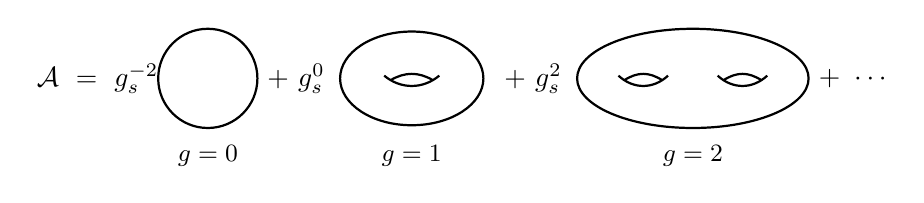
\begin{tikzpicture}[scale=0.7]
  \node at (-1.4,0) {$\mathcal{A}\ =\ g_s^{-2}$};
  \draw[thick] (0.6,0) circle (0.9);
  \node at (2.2,0) {$+\ g_s^{0}$};
  \begin{scope}[xshift=4.3cm]
    \draw[thick] (0,0) ellipse (1.3 and 0.85);
    \draw[thick] (-0.5,0.05) .. controls (-0.2,-0.2) and (0.2,-0.2) .. (0.5,0.05);
    \draw[thick] (-0.38,-0.03) .. controls (-0.12,0.12) and (0.12,0.12) .. (0.38,-0.03);
  \end{scope}
  \node at (6.5,0) {$+\ g_s^{2}$};
  \begin{scope}[xshift=9.4cm]
    \draw[thick] (0,0) ellipse (2.1 and 0.9);
    \foreach \c in {-0.9,0.9} {
      \draw[thick] (\c-0.45,0.05) .. controls (\c-0.18,-0.2) and (\c+0.18,-0.2) .. (\c+0.45,0.05);
      \draw[thick] (\c-0.34,-0.03) .. controls (\c-0.1,0.12) and (\c+0.1,0.12) .. (\c+0.34,-0.03);
    }
  \end{scope}
  \node at (12.3,0) {$+\ \cdots$};
  \node at (0.6,-1.4) {\small $g=0$};
  \node at (4.3,-1.4) {\small $g=1$};
  \node at (9.4,-1.4) {\small $g=2$};
\end{tikzpicture}
\caption{閉弦振幅（真空振幅）の種数展開．種数 $g$ の寄与は $g_s^{2g-2}$ で重みづけられる．}
\label{fig:ch13-genus-exp}
\end{figure}

\begin{physbox}[代数幾何が入り込む場所]
弦の摂動論は，Riemann 面のモジュライ空間 $\mathcal{M}_{g,n}$ とそのコンパクト化（Deligne--Mumford コンパクト化
$\overline{\mathcal{M}}_{g,n}$，結節点をもつ安定曲線を加える）の上の積分論である．
世界面が潰れていく極限（結節点の出現）は，場の理論の Feynman 図における伝搬関数の長い極限に対応する．
位相的弦理論ではこの積分が $\overline{\mathcal{M}}_{g,n}$ 上の交点数（Gromov--Witten 不変量）となり，
純粋に代数幾何的な量として計算される（第17章のミラー対称性）．
\end{physbox}

\exprob{ch13-pr-st}
$S:\tau\mapsto-1/\tau$，$T:\tau\mapsto\tau+1$ に対応する $\SL(2,\Z)$ の行列を書き，$S^2=-1$，$(ST)^3=-1$ を確かめよ．
また $\Img(-1/\tau) = \Img\tau/|\tau|^2$ を示し，測度 $d^2\tau/(\Img\tau)^2$ が $\SL(2,\Z)$ 不変であることを示せ．

\exprob{ch13-pr-cft}
自由ボソン $X$ の運動方程式 $\partial\bar\partial X=0$ の一般解が $X=X_L(z)+X_R(\bar z)$ と書けることを示し，
円筒座標 $z=e^{-iw}$，$w=\sigma^1+i\sigma^2$ で書いたとき，$X_L$，$X_R$ がそれぞれ左向き・右向きの波に対応することを説明せよ．

\section*{問題の解答}
\addcontentsline{toc}{section}{問題の解答}

\exsol{ch13-pr-p1}
$U_0\cap U_1=\{Z_0Z_1\neq0\}$ では $w=Z_0/Z_1=1/z$ であるから，$z=1/w$ より
\begin{equation*}
  dz = d\Bigl(\frac1w\Bigr) = -\frac{dw}{w^2}
\end{equation*}
である．$\PP^1$ 上の正則1形式 $\omega$ を考え，$U_0$ 上で $\omega=f(z)\,dz$（$f$ は $\C$ 上の正則関数），$U_1$ 上で $\omega=g(w)\,dw$（$g$ は $\C$ 上の正則関数）と書く．
重なりで
\begin{equation*}
  g(w)\,dw = f(z)\,dz = -\frac{f(1/w)}{w^2}\,dw,\qquad\text{すなわち}\qquad f(z) = -\frac{1}{z^2}\,g\Bigl(\frac1z\Bigr)\quad(z\neq0).
\end{equation*}
$g$ は $w=0$ の近傍で有界なので，$|z|\to\infty$ のとき $f(z)\to0$ である．したがって $f$ は $\C$ 上の有界な正則関数であり，
Liouville の定理により定数，しかも $\lim_{z\to\infty}f(z)=0$ からその定数は $0$ である．よって $f\equiv0$，$g\equiv0$，すなわち $\omega=0$．

以上より $\PP^1$ 上の正則1形式は $0$ しかなく，特に至るところ零でない正則1形式は存在しない．
（$dz$ そのものは $U_0$ 上では零にならないが，$w=0$ で2位の極 $-dw/w^2$ をもつ．これは $K_{\PP^1}\cong\OO(-2)$ の反映である．）

\exsol{ch13-pr-gl}
$A\in M_n(\C)$ を $\R$-線形写像 $\C^n\to\C^n$ とみたものを $A_\R\in M_{2n}(\R)$ と書く（実基底 $e_1,ie_1,\dots,e_n,ie_n$ をとる）．
$A\mapsto A_\R$ は同じ写像を実線形写像とみなすだけなので $(AB)_\R=A_\R B_\R$，$(1)_\R=1$ をみたす．したがって
可逆な $P$ に対し $\det(P^{-1}AP)_\R = \det(P_\R)^{-1}\det A_\R\det P_\R=\det A_\R$ である．

$A$ は複素数体上で上三角化できる：$A=PUP^{-1}$，$U$ は上三角で対角成分は $A$ の固有値 $\lambda_1,\dots,\lambda_n$．
上より $\det A_\R=\det U_\R$．$U$ が上三角であることは $Ue_j\in\C e_1+\cdots+\C e_j$ を意味するので，
実部分空間 $W_j=\R e_1\oplus\R ie_1\oplus\cdots\oplus\R e_j\oplus\R ie_j$ はすべて $U_\R$ で不変であり，
$U_\R$ は $2\times2$ ブロックの上三角行列になる．第 $j$ 対角ブロックは $W_j/W_{j-1}\cong\C$ 上の $\lambda_j$ 倍写像で，
$\lambda_j=a_j+ib_j$ とすると基底 $(e_j,ie_j)$ に関して
\begin{equation*}
  \begin{pmatrix} a_j & -b_j\\ b_j & a_j\end{pmatrix},\qquad \det = a_j^2+b_j^2 = |\lambda_j|^2
\end{equation*}
である（$\lambda_j e_j = a_je_j + b_j(ie_j)$，$\lambda_j(ie_j) = -b_je_j + a_j(ie_j)$）．ブロック上三角行列の行列式は対角ブロックの行列式の積なので
\begin{equation*}
  \det A_\R = \det U_\R = \prod_{j=1}^n|\lambda_j|^2 = \Bigl|\prod_{j=1}^n\lambda_j\Bigr|^2 = |\det A|^2 .
\end{equation*}

\exsol{ch13-pr-zero}
$f\not\equiv0$ としてよい（$f\equiv0$ なら零点集合は $\C^n$ で孤立点をもたない）．
$f$ の零点集合が孤立点 $p$ をもつと仮定する．すなわち $p$ を中心とする開球 $B$ で $\{f=0\}\cap B=\{p\}$ となるものがある．
このとき $1/f$ は $B\setminus\{p\}$ 上で正則である．$n\geq2$ なので $B\setminus\{p\}$ は連結であり（実 $2n\geq4$ 次元の球から1点を除いたもの），
Hartogs の拡張定理（定理\ref{thm:ch13-hartogs}，$U=B$，$K=\{p\}$）により $1/f$ は $B$ 上の正則関数 $g$ に拡張される．
$B\setminus\{p\}$ 上で $f g=1$ であり，両辺は $B$ 上連続なので $p$ でも $f(p)g(p)=1$．これは $f(p)=0$ に反する．
よって零点集合は孤立点を含まない．

\exsol{ch13-pr-aut}
$E=\C/\Lambda$ は連結なコンパクト Riemann 面，$f:E\to\PP^1$ を定数でない正則写像とする．

\textbf{開写像性}：$E$ は連結なので，一致の定理により $f$ はどの開集合上でも定数でない．$p\in E$ の近くで局所座標をとり
$f(p)$ を原点とする $\PP^1$ の座標で $f$ を表すと，$f(z)=z^k u(z)$（$k\geq1$，$u(0)\neq0$）と書ける．
$u$ の $k$ 乗根 $v$（$v^k=u$，$p$ の近傍で正則）をとれば $\zeta=zv(z)$ は新しい局所座標で $f=\zeta^k$ となり，
$\zeta\mapsto\zeta^k$ は開写像なので $f$ は $p$ の近傍を $f(p)$ の近傍に写す．よって $f(E)$ は $\PP^1$ の開集合である．

\textbf{閉性}：$E$ はコンパクトなので $f(E)$ はコンパクトであり，Hausdorff 空間 $\PP^1$ の中で閉集合である．

$f(E)$ は空でない開かつ閉な部分集合で，$\PP^1$ は連結だから $f(E)=\PP^1$．すなわち $f$ は全射である．
（同じ議論で，コンパクト Riemann 面の間の定数でない正則写像は常に全射である．）

\exsol{ch13-pr-cusp}
\textbf{全単射性}：$(t^2)^3=(t^3)^2$ なので $\nu(\C)\subset C$．逆に $(z,w)\in C$ とする．$z=0$ なら $w^2=0$ より $w=0$ で，$t=0$ がただ一つの逆像である．
$z\neq0$ なら $t=w/z$ とおくと $t^2=w^2/z^2=z^3/z^2=z$，$t^3=t\cdot t^2=w$ であり，逆に $\nu(t)=(z,w)$ なら $t=t^3/t^2=w/z$ と一意に決まる．
よって $\nu$ は全単射で，逆写像は
\begin{equation*}
  \nu^{-1}(z,w)=\begin{cases} w/z & (z\neq0)\\ 0 & (z=w=0)\end{cases}
\end{equation*}
である．$\nu$ は連続で，$\nu^{-1}$ も連続である：$z\neq0$ では明らかであり，原点では $|\nu^{-1}(z,w)|=|z|^{1/2}\to0$（$t^2=z$ より）．よって $\nu$ は同相写像である．

\textbf{逆写像は正則でない}：$\nu^{-1}$ が $C$ 上の正則写像だとすると，$0$ の近傍で $\C^2$ 上の正則関数 $G(z,w)$ の制限として $\nu^{-1}=G|_C$ と書ける
（局所モデル上の正則関数の定義）．すると $G(t^2,t^3)=t$ が成り立つ．$t$ で微分して $t=0$ とおくと，
$\nu'(0)=(2t,3t^2)|_{t=0}=(0,0)$ より左辺は $\partial_zG\cdot0+\partial_wG\cdot0=0$，右辺は $1$ となり矛盾．
（下の $\nu^*$ の像の記述からも，$t\notin\Img\nu^*$ として分かる．）

\textbf{$\nu^*$ の像}：$\OO_{C,0}$ の元は原点での収束冪級数 $G(z,w)\in\C\{z,w\}$ の類であり，$\nu^*G(t)=G(t^2,t^3)$．
単項式は $\nu^*(z^aw^b)=t^{2a+3b}$ に写り，$2a+3b$（$a,b\geq0$）のとる値は $0,2,3,4,5,\dots$ で $1$ だけをとらない．
したがって $\nu^*G$ は $t^1$ の係数が $0$ の収束冪級数であり，$\Img\nu^*\subset\{\sum_n c_nt^n:c_1=0\}$．
逆に $h(t)=c_0+\sum_{n\geq2}c_nt^n$ が収束冪級数（ある $r>0$ で $\sum|c_n|r^n<\infty$）なら，偶数次 $2k=2\cdot k$ と奇数次 $2k+3$ に分けて
\begin{equation*}
  G(z,w) = \sum_{k\geq0}c_{2k}z^k + w\sum_{k\geq0}c_{2k+3}z^k
\end{equation*}
とおけば，これは $|z|<r^2$ で収束し $G(t^2,t^3)=h(t)$ をみたす．よって
\begin{equation*}
  \Img\nu^* = \Bigl\{\sum_n c_nt^n\in\C\{t\} : c_1=0\Bigr\} = \C\{t^2,t^3\}
\end{equation*}
である（右の等号は，$t^2,t^3$ の収束冪級数で書けるものがちょうど $c_1=0$ の級数であることを今示したことによる）．
$\Img\nu^*\subsetneq\OO_{\C,0}=\C\{t\}$ であり，欠けている $t$ こそ逆写像の座標関数である．
$\nu$ は同相だが局所環の同型を誘導しない，というのが「尖点は特異点」であることの代数的表現である．

\exsol{ch13-pr-chow}
$\C^2\subset\PP^2$ を $(z,w)\mapsto[1:z:w]$（同次座標 $[Z_0:Z_1:Z_2]$，無限遠直線 $L_\infty=\{Z_0=0\}$）で埋め込み，
$A=\{w=e^z\}$ の $\PP^2$ での閉包を $\bar A$ とする．$A$ は $\C^2$ で閉なので $\bar A\cap\C^2=A$ である．

\textbf{$[0:1:0]\in\bar A$}：$A$ の点 $(2\pi ik,1)$（$k\in\Z$）は $[1:2\pi ik:1]=[1/(2\pi ik):1:1/(2\pi ik)]$ であり，$k\to\infty$ で $[0:1:0]$ に収束する．
（実際には $L_\infty$ のすべての点が $\bar A$ に含まれる．たとえば $z\to-\infty$（実）で $[1:z:e^z]\to[0:1:0]$，$z\to+\infty$ で $\to[0:0:1]$ である．）

\textbf{$\bar A$ は解析的集合でない}：直線 $\ell=\{Z_2=Z_0\}$（$\C^2$ 内では $w=1$）を考える．
もし $\bar A$ が $\PP^2$ の閉解析的部分集合なら，その定義関数を $\ell\cong\PP^1$ に制限して，$\bar A\cap\ell$ は $\ell$ の閉解析的部分集合となる．
連結な1次元複素多様体 $\ell$ の解析的部分集合 $S$ は，$\ell$ 全体であるか離散集合（$\ell$ はコンパクトなので有限集合）である．
実際，「$p$ の近傍で $S$ の局所定義関数がすべて恒等的に $0$」となる点 $p$ の集合は開であり，一致の定理により閉でもある．
それが空なら，$S$ の各点で少なくとも1つの定義関数は恒等的に $0$ でない1変数正則関数なので，その零点は孤立している．
ところが $\bar A\cap\ell$ は無限個の点 $(2\pi ik,1)$ を含むので有限でなく，一方 $(1,1)\in\ell$ は $e^1\neq1$ より $\bar A$ に属さないので $\ell$ 全体でもない．
これは矛盾であり，$\bar A$ は $\PP^2$ の解析的集合でない．

したがって $A$ は「$\PP^2$ の閉解析的部分集合の $\C^2$ への制限」の形をしておらず，Chow の定理の仮定をみたさない．
Chow の定理は $\PP^n$ 全体で閉な解析的集合についての主張であり，$A$ は無限遠直線に向かって無限回巻きつき（$e^z$ の本質的特異点），
閉包が無限遠で解析的に閉じない．したがって矛盾はない．
逆に言えば，もし $A$ が代数的なら $\bar A$ は射影代数曲線（とくに解析的）になるはずであり，例\ref{ex:ch13-nonalg} の結論は Chow の定理と整合する．

\exsol{ch13-pr-hopf}
写像
\begin{equation*}
  \Psi:\C^2\setminus\{0\}\to S^3\times\R,\qquad z\mapsto\Bigl(\frac{z}{|z|},\ \log_2|z|\Bigr)
\end{equation*}
を考える（$S^3=\{u\in\C^2:|u|=1\}$）．$|z|$ は $z\neq0$ で滑らかで正なので $\Psi$ は滑らかであり，逆写像 $(u,t)\mapsto 2^tu$ も滑らかだから，$\Psi$ は微分同相である．
生成元 $\gamma:z\mapsto2z$ は
\begin{equation*}
  \Psi(2z) = \Bigl(\frac{z}{|z|},\ \log_2|z|+1\Bigr)
\end{equation*}
より，$S^3\times\R$ 上の $(u,t)\mapsto(u,t+1)$ に対応する．$\Z$ のこの作用は自由かつ真性不連続であり，商は
\begin{equation*}
  (S^3\times\R)/\Z = S^3\times(\R/\Z)\cong S^3\times S^1
\end{equation*}
である．$\Psi$ は $\Z$ 作用と可換な微分同相なので，商空間の間の微分同相 $X=(\C^2\setminus\{0\})/\langle\gamma\rangle\cong S^1\times S^3$ を誘導する
（商写像はどちらも局所微分同相である）．
なお $\gamma$ は正則なので $X$ はコンパクト複素多様体であり，Künneth の公式から $b_1(X)=b_1(S^1)+b_1(S^3)=1$ となる（本文の「$b_1=1$ が奇数なので Kähler でない」）．

\exsol{ch13-pr-genus}
種数公式（定理\ref{thm:ch13-genus-formula}）より
\begin{equation*}
  \chi = 2-2g = 2-(d-1)(d-2) = 2-(d^2-3d+2) = -d^2+3d .
\end{equation*}
（$d=1,2$ で $\chi=2$（球面），$d=3$ で $\chi=0$（トーラス）であり，前の表と合う．）

$d=4$ では $g=(4-1)(4-2)/2=3$，$\chi=-16+12=-4$ である．Fermat 曲線 $F=X^4+Y^4+Z^4$ は，
$\partial F/\partial X=4X^3$，$\partial F/\partial Y=4Y^3$，$\partial F/\partial Z=4Z^3$ が同時に消えるのは $X=Y=Z=0$ のみで，これは $\PP^2$ の点ではないから非特異である．
よってその種数は $3$ である．

\exsol{ch13-pr-wp}
$\Lambda=\Z+\Z i$ では $i\Lambda=\Lambda$ であり，$\lambda\mapsto i\lambda$ は $\Lambda\setminus\{0\}$ の全単射である．
$\sum_{\lambda\neq0}|\lambda|^{-6}<\infty$ なので級数は絶対収束し，項の並べ替えが許される．したがって
\begin{equation*}
  \sum_{\lambda\neq0}\frac1{\lambda^6} = \sum_{\lambda\neq0}\frac1{(i\lambda)^6} = i^{-6}\sum_{\lambda\neq0}\frac1{\lambda^6} = -\sum_{\lambda\neq0}\frac1{\lambda^6}
\end{equation*}
となり，$\sum\lambda^{-6}=0$，すなわち $g_3=0$．
（同じ置換で $\sum\lambda^{-4}=i^{-4}\sum\lambda^{-4}$ となり，$g_2$ については何の制約も出ない．）

$g_3=0$ のとき判別式は $\Delta=g_2^3-27g_3^2=g_2^3$ であり，楕円曲線は非特異だから $\Delta\neq0$，とくに $g_2\neq0$．よって
\begin{equation*}
  j(i) = 1728\,\frac{g_2^3}{g_2^3-0} = 1728 .
\end{equation*}
（$\tau=i$ は $S:\tau\mapsto-1/\tau$ の固定点であり，正方格子は位数4の自己同型 $z\mapsto iz$ をもつ特別な楕円曲線 $y^2=4x^3-g_2x$ を与える．）

\exsol{ch13-pr-st}
\textbf{行列と関係式}：$\tau\mapsto(a\tau+b)/(c\tau+d)$ に行列 $\begin{pmatrix}a&b\\c&d\end{pmatrix}$ を対応させると
\begin{equation*}
  S=\begin{pmatrix}0&-1\\1&0\end{pmatrix},\qquad T=\begin{pmatrix}1&1\\0&1\end{pmatrix}
\end{equation*}
である（$S\tau=(0\cdot\tau-1)/(\tau+0)=-1/\tau$）．いずれも行列式 $1$ である．計算すると
\begin{gather*}
  S^2=\begin{pmatrix}0&-1\\1&0\end{pmatrix}^2=\begin{pmatrix}-1&0\\0&-1\end{pmatrix}=-1,\qquad
  ST=\begin{pmatrix}0&-1\\1&1\end{pmatrix},\\
  (ST)^2=\begin{pmatrix}-1&-1\\1&0\end{pmatrix},\qquad
  (ST)^3=\begin{pmatrix}-1&-1\\1&0\end{pmatrix}\begin{pmatrix}0&-1\\1&1\end{pmatrix}=\begin{pmatrix}-1&0\\0&-1\end{pmatrix}=-1 .
\end{gather*}
$-1$ は $\tau$ に自明に作用するので，$\mathbb{H}$ への作用としては $S^2=(ST)^3=\mathrm{id}$ である．

\textbf{虚部の変換}：一般に $\gamma=\begin{pmatrix}a&b\\c&d\end{pmatrix}\in\SL(2,\Z)$，$\tau'=\gamma\tau$ に対し
\begin{equation*}
  \tau' = \frac{(a\tau+b)(c\bar\tau+d)}{|c\tau+d|^2} = \frac{ac|\tau|^2+ad\tau+bc\bar\tau+bd}{|c\tau+d|^2},\qquad
  \Img\tau' = \frac{(ad-bc)\Img\tau}{|c\tau+d|^2} = \frac{\Img\tau}{|c\tau+d|^2}.
\end{equation*}
$S$（$c=1,d=0$）では $\Img(-1/\tau)=\Img\tau/|\tau|^2$．直接にも $-1/\tau=-\bar\tau/|\tau|^2$ の虚部は $\Img\tau/|\tau|^2$ である．

\textbf{測度の不変性}：$\tau'$ は $\tau$ の正則関数で
\begin{equation*}
  \frac{d\tau'}{d\tau} = \frac{a(c\tau+d)-c(a\tau+b)}{(c\tau+d)^2} = \frac{1}{(c\tau+d)^2}.
\end{equation*}
正則写像の実 Jacobi 行列式は $|d\tau'/d\tau|^2$ であるから（問\ref{ch13-pr-gl} の $n=1$ の場合），$d^2\tau=d(\Re\tau)\,d(\Img\tau)$ は
$d^2\tau' = |c\tau+d|^{-4}d^2\tau$ と変換する．したがって
\begin{equation*}
  \frac{d^2\tau'}{(\Img\tau')^2} = \frac{|c\tau+d|^{-4}\,d^2\tau}{|c\tau+d|^{-4}(\Img\tau)^2} = \frac{d^2\tau}{(\Img\tau)^2}
\end{equation*}
であり，測度 $d^2\tau/(\Img\tau)^2$ は $\SL(2,\Z)$（さらに $\SL(2,\R)$）不変である．とくに $S,T$ で不変である．

\exsol{ch13-pr-cft}
\textbf{一般解}：$X$ を（単連結な）領域 $U\subset\C$ 上の解とする．$\bar\partial(\partial X)=0$ より $f:=\partial X$ は正則関数である．
$U$ は単連結なので $f$ の原始関数 $X_L$（$X_L'=f$，正則）がとれる．$Y:=X-X_L$ とおくと，$X_L$ は正則なので $\partial X_L = X_L' = f$ であり，
\begin{equation*}
  \partial Y = \partial X - \partial X_L = f - f = 0 .
\end{equation*}
すなわち $Y$ は反正則関数 $X_R(\bar z)$ である．よって $X=X_L(z)+X_R(\bar z)$．逆にこの形の関数は明らかに $\partial\bar\partial X=0$ をみたす．
（$X$ が実なら $\overline{\partial X}=\bar\partial X$ なので，$X_R$ は $\overline{X_L}$ に定数を加えたものにとれる．）

$U=\C^*$ のような単連結でない領域では，$f=\partial X=\sum_n a_nz^{n-1}$（Laurent 展開）の $z^{-1}$ の項だけは1価な原始関数をもたず，$\log z$ を生む．
しかし $X$ が1価なら $\log z$ と $\log\bar z$ が組になって $\log|z|^2$ となり，
\begin{equation*}
  X = x_0 + c\log|z|^2 + \sum_{n\neq0}\bigl(a_nz^{-n}+\tilde a_n\bar z^{-n}\bigr)
\end{equation*}
の形になる．$\log|z|^2=\log z+\log\bar z$ を左右に半分ずつ配れば，多価性を除いて同じ分解が成り立つ．

\textbf{円筒座標}：$w=\sigma^1+i\sigma^2$，$\sigma^1\sim\sigma^1+2\pi$ とすると，$z=e^{-iw}=e^{\sigma^2}e^{-i\sigma^1}$ は円筒 $\R\times S^1$ から $\C^*$ への双正則写像であり，
$|z|=e^{\sigma^2}$ より Euclid 時間 $\sigma^2$ は動径方向（$\sigma^2\to-\infty$ が原点）に，空間方向 $\sigma^1$ は角度方向に移る．
$z$ は $w$ の正則関数なので，$X_L(z)$ は $w$ の正則関数，$X_R(\bar z)$ は $\bar w$ の正則関数である．上の展開は
\begin{equation*}
  z^{-n}=e^{in w}=e^{in\sigma^1-n\sigma^2},\qquad \bar z^{-n}=e^{-in\bar w}=e^{-in\sigma^1-n\sigma^2},\qquad \log|z|^2=2\sigma^2
\end{equation*}
となり，$\log|z|^2$ の項は重心の時間発展（運動量）を表す．

Minkowski 署名に戻すため $\sigma^2=i\sigma^0$（$\sigma^0$ は実時間）とおくと
\begin{equation*}
  w=\sigma^1-\sigma^0,\qquad \bar w=\sigma^1+\sigma^0
\end{equation*}
である．したがって $X_L$ は $\sigma^1-\sigma^0$ だけの関数，$X_R$ は $\sigma^1+\sigma^0$ だけの関数であり，
前者は形を保ったまま $\sigma^1$ の正の向きに，後者は負の向きに，ともに光速で弦に沿って伝わる波である
（$e^{in(\sigma^1-\sigma^0)}$ と $e^{-in(\sigma^1+\sigma^0)}$ が振動モード）．
こうして正則部分と反正則部分は互いに逆向きに独立に進む波に対応する．どちらを「左向き」と呼ぶかは $\sigma^1$ 軸の向き（と Wick 回転の符号）の約束によるが，
弦理論の標準的な約束（Polchinski）に従って正則部分 $X_L$ を左向き，反正則部分 $X_R$ を右向きの波と呼ぶ．
本質的な内容は，$\partial\bar\partial X=0$ が $z,\bar z$ について分離することが，Minkowski 署名での光錐座標 $\sigma^\pm$ についての分離 $\partial_+\partial_-X=0$
（波動方程式の d'Alembert 解）そのものであるという点である．
